\documentclass{article}
\usepackage[utf8]{inputenc}
\usepackage[french]{babel}
\usepackage{amssymb}
\usepackage{stmaryrd}
\usepackage{enumitem}
\usepackage{amsmath}
\usepackage{array}
\usepackage[left=2cm,right=2cm,top=2cm,bottom=2cm]{geometry}
\usepackage[T1]{fontenc}
\setlength\parindent{0pt}
\usepackage{graphicx}
\usepackage[ddmmyyyy]{datetime}
\usepackage[backend=biber]{biblatex}
\addbibresource{ref.bib}
\usepackage{booktabs}
\usepackage{float}
\usepackage{setspace}
\usepackage{hyperref}
\hypersetup{
    colorlinks=true,
    linkcolor=blue,
    filecolor=magenta,      
    urlcolor=cyan,
}
\usepackage{easytable}
\usepackage{adjustbox}
\usepackage{listings}
\lstdefinelanguage{Matlab}%
  {morekeywords={matlab2tikz},
   morekeywords=[2]{1}, 
   morekeywords=[3]{xlim,ylim,clim,iter},
   morekeywords=[4]{x,y,scatter,contour,imagesc,addplot3},
   morecomment=[l][\color{blue}]{...},%
   morestring=[m]',%
   morestring=[m]"%
  }[keywords,comments,strings]

\lstset{%
  language=Matlab,%
  breaklines=true,%
  morekeywords={matlab2tikz},
  keywordstyle=\color{blue},%
  morekeywords=[2]{1}, keywordstyle=[2]{\color{black}},
  identifierstyle=\color{black},%
  stringstyle=\color{mylilas},
  commentstyle=\color{mygreen},%
  showstringspaces=false,
  numbers=left,%
  numberstyle={\tiny \color{black}},
  numbersep=9pt,
  emph=[1]{for,end,break},emphstyle=[1]\color{red},
}

\hypersetup{
    colorlinks=true,
    linkcolor=black,  % Changer la couleur ici
    filecolor=magenta,      
    urlcolor=cyan,
}

\usepackage{tikz}
\usetikzlibrary{calc}

\renewcommand{\dateseparator}{/}

\usepackage{fancyhdr}
\usepackage{lastpage}

\pagestyle{fancy}
\renewcommand\headrulewidth{1pt}
\renewcommand\footrulewidth{1pt}
\geometry{headsep=1.1cm}

\newtheorem{theorem}{Théorème}[subsection]
\newtheorem{corollary}{Corollaire}[theorem]
\newtheorem{lemma}[theorem]{Lemme}
\newtheorem{definition}{Définition}[subsection]
\newtheorem{proposition}{Proposition}[section]

\fancyhead[L]{
\includegraphics[width=0.1\columnwidth]{./logo}~}
\fancyfoot[L]{\textsc{CentraleSupélec - 2A}}
\fancyhead[R]{\textsc{EI - Contrôle de la pollution acoustique}}
\fancyfoot[C]{\thepage/\pageref{LastPage}}
\fancyfoot[R]{\textsc{\today}}

\usepackage{xcolor}
\usepackage{piton}
\usepackage{tcolorbox}
\newcommand{\Tr}{\operatorname{Tr}}
\newcommand{\Arg}{\operatorname{Arg}}

%====================== INFORMATION ET REGLES ======================

%rajouter les numérotation pour les \paragraphe et \subparagraphe
\setcounter{secnumdepth}{4}
\setcounter{tocdepth}{4}

%======================== DEBUT DU DOCUMENT ========================

\begin{document}

% \NewPitonEnvironment{Python}{O{}}{\PitonOptions{#1}}{}
\PitonOptions{break-lines, indent-broken-lines}

\NewPitonEnvironment{Python}{}
  {\begin{tcolorbox}[breakable]}
  {\end{tcolorbox}}


%régler l'espacement entre les lignes
\newcommand{\HRule}{\rule{\linewidth}{0.5mm}}

%page de garde
\begin{titlepage}
\begin{center}

% Upper part of the page. The '~' is needed because only works if a paragraph has started.

\LARGE \textsc{2EL1740: Algèbre \& Cryptologie}

\vspace{0.2cm}

\Large \textsc{CentraleSupélec - 2A}

\vspace{0.3cm}

% Title
\HRule \\[0.4cm]

{\huge \bfseries Challenge 4\\
[0.2cm]}

\HRule \\[0.4cm]

\vspace{2cm}

\textsc{\today}

\vspace{2cm}


\includegraphics[width=0.4\columnwidth]{./logo}~\\[3cm]

% Author and supervisor
\begin{minipage}{0.4\textwidth}
\begin{spacing}{1.125}
\begin{center}
    Raphaël \testsc{PAIN DIT HERMIER}\\
    Alexis \testsc{LOMBARD-GAILLARD}\\
    Edward \testsc{LUCYSZYN}
\end{center}
\end{spacing}
\end{minipage}

\vfill

\end{center}
\end{titlepage}

%page blanche
%\newpage
%~
%ne pas numéroter cette page
\thispagestyle{empty}


\tableofcontents
\thispagestyle{empty}
% \setcounter{page}{1}
%ne pas numéroter le sommaire

%\newpage

%espacement entre les lignes d'un tableau
\renewcommand{\arraystretch}{1.5}

%====================== INCLUSION DES PARTIES ======================

~
\thispagestyle{empty}
%recommencer la numérotation des pages à "1"
\setcounter{page}{0}

\newpage

\section{Introduction}

\subsection{Contexte}

Nous sommes \textsc{Nabilou}, spécialisés dans l'innovation acoustique de l'industrie aérospatiale ! Notre mission consiste à redéfinir l'avenir des voyages aériens en minimisant le bruit à l'intérieur des réacteurs d'aéronefs pour améliorer les conditions des passagers et des acteurs extérieurs.\\ \\
En effet, les moteurs d'aéronefs génèrent un niveau sonore considérable, et nous avons relevé ce défi avec détermination. Avec une équipe dédiée et une approche novatrice, nous utilisons des liners acoustiques disposés de manière optimale, assurant ainsi le meilleur compromis entre l'efficacité et le coût !\\ \\
Notre travail s'inscrit dans la continuité du cours de ST5 sur le contrôle de la pollution acoustique. Parmi nos six membres, trois d'entre eux participent à un projet de formation à la recherche sur l'équation de Helmholtz convectée à CentraleSupélec en partenariat avec l'ONERA. C'est pourquoi, au sein de ce rapport, l'équipe théorique composée de deux membres s'est chargée d'une étude plus approfondie que la normale, utilisant ladite équation d'Helmholtz convectée. Enfin, les quatre autres membres du groupe ont réalisé l'étude de la partie numérique.

\subsection{Objectifs et défis}

Afin de proposer la meilleure solution pour réduire le bruit des réacteurs, nous avons dû répondre à différents objectifs tout au long de ces cinq jours. Pour l'équipe numérique :

\begin{itemize}
    \item Choix de la forme des liners ;
    \item Choix du matériaux des liners ;
    \item Optimisation de la disposition des liners ;
    \item Optimisation multi-fréquentielle ;
    \item Recherche d'autres méthodes d'optimisation \item Optimisation de la quantité de matériaux ;
    \item Description de la solution choisie ;
    \item Comparaison de la solution choisie avec une paroi complètement absorbante.
\end{itemize}
Et pour l'équipe théorique :
\begin{itemize}
    \item S'assurer théoriquement de la validité des équations d'onde utilisées ;
    \item Montrer le caractère bien posé des équations variationnelles obtenues ;
    \item Montrer la continuité de l'énergie acoustique (qui dépend de la distribution de matériau choisie) ;
    \item Montrer l'existence de distributions optimales admissibles pour une quantité de matériau fixée (minimisant l'énergie acoustique) ;
    \item Trouver explicitement une expression de la dérivée de l'énergie acoustique satisfaisante.
\end{itemize}

\newpage

\section{Introduction au problème numérique}

Les domaines de l'électromagnétisme et de l'acoustique sont régis par de nombreuses équations aux dérivées partielles faisant place à des systèmes parfois non solvables analytiquement. Cela constitue donc un défi majeur en mathématiques appliquées. Pouvoir résoudre ces équations numériquement est par conséquent essentiel à l'étude de la propagation d'un son, et donc nécessaire pour diminuer le bruit dans un réacteur d'avion.\\ \\
Dans un premier temps, nous expliquerons le problème que nous avons dû résoudre numériquement. Puis dans un second temps, nous étudierons le fonctionnement des algorithmes permettant de calculer l'énergie minimale dans le domaine. Enfin, nous analyserons les différents résultats obtenus.

\subsection{Présentation du problème}

Considérons un volume rectangulaire de 1m horizontalement et de 2m verticalement, comportant $N\times2N$ quadrangles. Le matériau poreux est déposé sur la surface au milieu, qui est plus au moins irrégulière en fonction du niveau de fractale.

\begin{figure}[H]
    \centering
    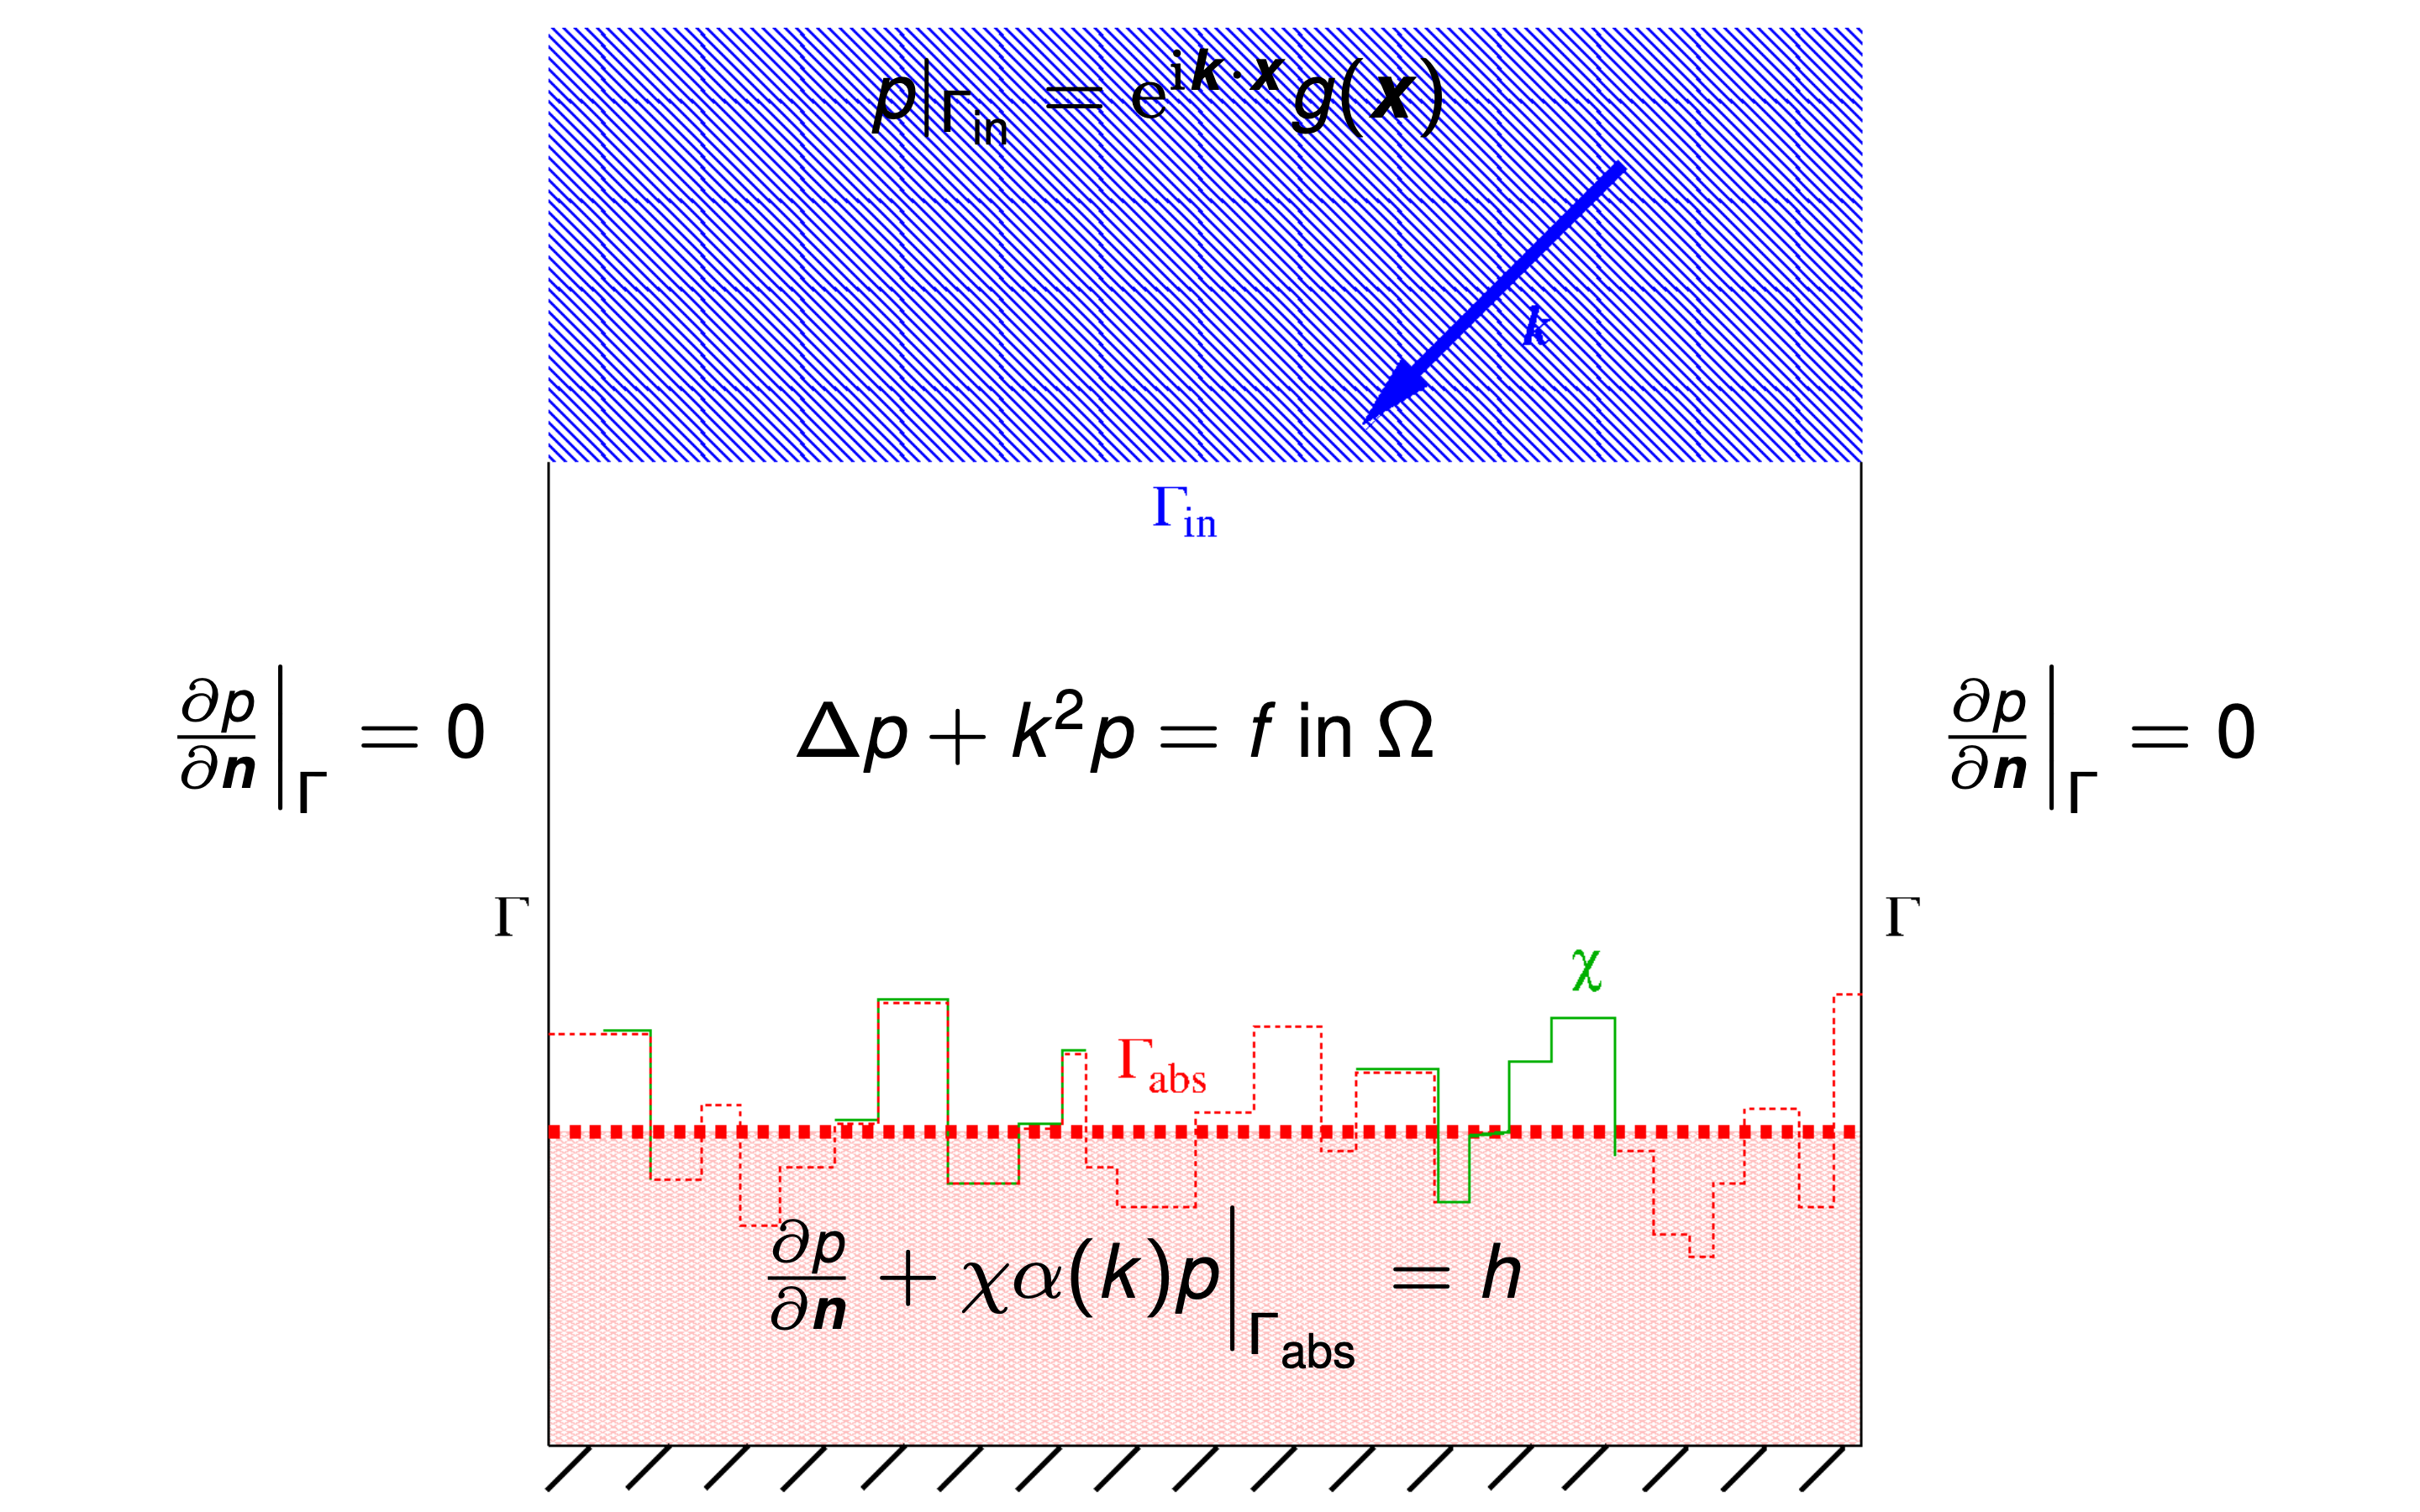
\includegraphics[width=0.8\linewidth]{rapport/numerique/assets/probleme.png}
    \caption{Modélisation du problème dans notre domaine}
    \label{fig:enter-label}
\end{figure}

On impose des conditions de Dirichlet pour la surface supérieure, des conditions de Neumann pour les surfaces latérales et des conditions de Robin pour la paroi du réacteur (surface inférieure). Le système d'équation dans le domaine est donc le suivant:
\begin{equation}
    \tag{$P_\chi$}
    \begin{cases}
    \Delta p + k^2 p = 0 \text{ dans } \Omega \\
    p = g_{in} \text{ sur } \Gamma_{in} \\
    \displaystyle \frac{\partial p}{\partial n} = 0 \text{ sur } \Gamma \\[5pt]
    \displaystyle \frac{\partial p}{\partial n} + \alpha \chi p = 0 \text{ sur } \Gamma_{abs}
    \end{cases} 
\end{equation}
où $p$ est l'inconnue du système, $\alpha$ est le coefficient d'absorption du liner et $\chi$ représente la répartition de matériaux poreux à la frontière. \\ \\
La quantité de matériaux est $$\beta = \displaystyle \displaystyle \int_{\Gamma_{abs}}\chi dS.$$
L'objectif final du projet est de trouver le niveau de fractale, le matériau et la quantité la plus faible de matériaux $\beta$ permettant de minimiser l'énergie dans le réacteur et donc le bruit dans le réacteur. \\ \\
L'énergie totale dans le domaine est donnée par la formule:
$$J(\chi) := \int_\Omega |p_\chi|^2dx$$
où $p_\chi$ est la solution du système $(P_\chi)$.

\subsection{Structure du code}

Dans le code, présent dans le fichier accompagnant ce rapport, nous trouvons cinq fichiers Python. \\ \\
Les trois premiers, \texttt{preprocessing.py}, \texttt{processing.py}, \texttt{postprocessing.py} sont des "boites noires" qui nous ont été fournies et qui n'ont pas été modifiées. Le premier fichier, \texttt{preprocessing.py} sert principalement à créer la fractale et définit des fonctions de base. Le deuxième, \texttt{processing.py}, a pour but de résoudre l'équation d'Helmholtz dans le domaine. Enfin, \texttt{postprocessing.py}, sert uniquement à créer différents graphiques montrant l'énergie dans le domaine, ou encore $\chi$, la disposition de notre matériaux poreux sur la frontière.\\ \\
L'autre fichier \texttt{\_env.py}, permet d'identifier la nature de chaque point du maillage. La liste qui traduit la nature de tous les points s'appelle \texttt{domain\_omega}, et attribue à chaque point une valeur entière non nulle entre $-2$ et $3$ en fonction de si ce point correspond à une condition de Dirichlet, de Robin, de Neumann, à l'intérieur du domaine ou à l'extérieur.\\ \\
Enfin, le dernier fichier, que nous avons complété est \texttt{main.py}. Ce fichier comporte la fonction permettant de calculer l'énergie dans le domaine et l'algorithme d'optimisation associé.


\newpage

\section{Écriture du code}

Cette partie explique toutes les fonctions que nous avons écrites, complétées ou rajoutées dans le fichier \\ \texttt{demo\_control\_polycopie2023.py}.

\subsection{Calcul de l'énergie}

\subsubsection{Description de l'algorithme}

Tout d'abord, la première fonction que nous avons écrite est celle permettant de calculer l'énergie $J(\chi) := \int_\Omega |p_\chi|^2dx$. Cette fonction est appelée \texttt{your\_compute\_objective\_function} dans le code. Afin d'approcher l'intégrale permettant de calculer l'énergie, nous utilisons l'algorithme suivant:

\begin{itemize}
    \item Prendre un point du maillage qui possède un voisin à droite et en bas;
    \item Vérifier si le carré formé par le point initial, son voisin en bas, son voisin à droite et son voisin en bas à droite est dans l'intérieur du domaine;
    \item Si c'est le cas, calculer la moyenne de la valeur absolue au carré des points du carré;
    \item Multiplier cette moyenne par l'aire du carré, cela nous donne une approximation de l'énergie dans le carré;
    \item Faire ceci pour tous les points qui ont un voisin à droite et en bas.
\end{itemize}

Cette formule de l'approximation de l'aire de la courbe d'une fonction à deux variables vient de \cite{4} et s'écrit, pour une fonction $f$ définie sur les coins du rectangle $[a, b]\times[c, d]$ et qui satisfait certaines conditions:
$$\displaystyle \int_a^b \int_c^d f(x,y)dy dx = [f(a,c) + f(a, d) + f(b, c) + f(b, d)]\frac{(b-a)(d-c)}{4} + E(f)$$ avec $E(f)$ l'erreur qui dépend des conditions sur $f$.\\ \\
De plus, pour vérifier que le carré considéré est bien dans le domaine et non pas à l'extérieur, il faut qu'au minimum un des points du carré soit à l'intérieur. Cette condition permet de bien prendre en compte l'énergie qui entre la frontière et l'intérieur dans la discrétisation.

\subsubsection{Implémentation en Python}

\begin{Python}
def your_compute_objective_function(domain_omega, u, spacestep):
    energy = 0.0
    for i in range(0, M-1):
        for j in range(0, N-1):
            if domain_omega[i, j] == _env.NODE_INTERIOR or domain_omega[i+1, j] == _env.NODE_INTERIOR or domain_omega[i, j+1] == _env.NODE_INTERIOR or domain_omega[i+1, j+1] == _env.NODE_INTERIOR:
                energy += (numpy.abs(u[i, j])**2 + numpy.abs(u[i+1, j])**2 + numpy.abs(u[i, j+1])**2 + numpy.abs(u[i+1, j+1])**2)*spacestep*spacestep/4
    return energy
\end{Python}

\subsection{Algorithme du gradient}

\subsubsection{Présentation théorique}

Afin d'optimiser de trouver la configuration optimale pour laquelle l'énergie est la plus basse dans notre domaine, il faut que nous minimisions l'énergie. Vu que cette dernière dépend de plusieurs variables, nous devons employée une méthode valable pour plusieurs variables. La méthode employée a été celle de la méthode de descente de gradient. Cela consiste à minimiser une fonction réelle différentiable dans un espace euclidien. \\ \\
Dans notre problème la fonction à minimiser est $ \chi \mapsto J(\chi)$. $J$ est bien différentiable au sens de Fréchet avec $J'(\chi) : L^{\infty}(\Gamma_{abs}) \to L^1(\Gamma_{abs})$ telle que:
$$J(\chi + \chi_0) = J(\chi) + \langle J'(\chi), \chi_0 \rangle + o(\chi_0)\,, \lim_{||\chi_0||_{\infty} \to 0} \displaystyle \frac{|o(\chi_0)|}{||\chi_0||_{\infty}} = 0.$$
L'algorithme du gradient va nous amener à considérer la suite $(\chi^{(n)})_{n \ge 0}$ définie par la relation:
$$ \chi^{(k+1)} = \mathcal{P}_{\ell_k}\big[\chi^{(k)} - \mu_k J'(\chi^{(k)})\big]$$
où $\mathcal{P}_{\ell_k}$ est un projecteur visant à restreindre $\chi^{(k)} - \mu_k J'(\chi^{(k)})$ dans $[0, 1]$ et garantir $\beta = \displaystyle \int_{\Gamma_{abs}}\chi^{(k+1)}  dS$, et où $\mu_k > 0$ est un paramètre, recalculé à chaque étape, défini comme le taux d'apprentissage. Nous parlerons de $\mathcal{P}_{\ell_k}$ juste après.\\ \\
Si à l'itération $k+1$ nous n'arrivons pas à diminuer l'énergie par rapport à l'itération $k$, nous divisions par $2$ le taux d'apprentissage $\mu_k$ et nous recalculons $\chi^{(k+1)}$. Cependant si l'énergie est bel et bien diminuée, alors on augmente $\mu_k$. Le pseudo code de l'algorithme est en présent en Figure 2. 

\begin{figure}[H]
    \centering
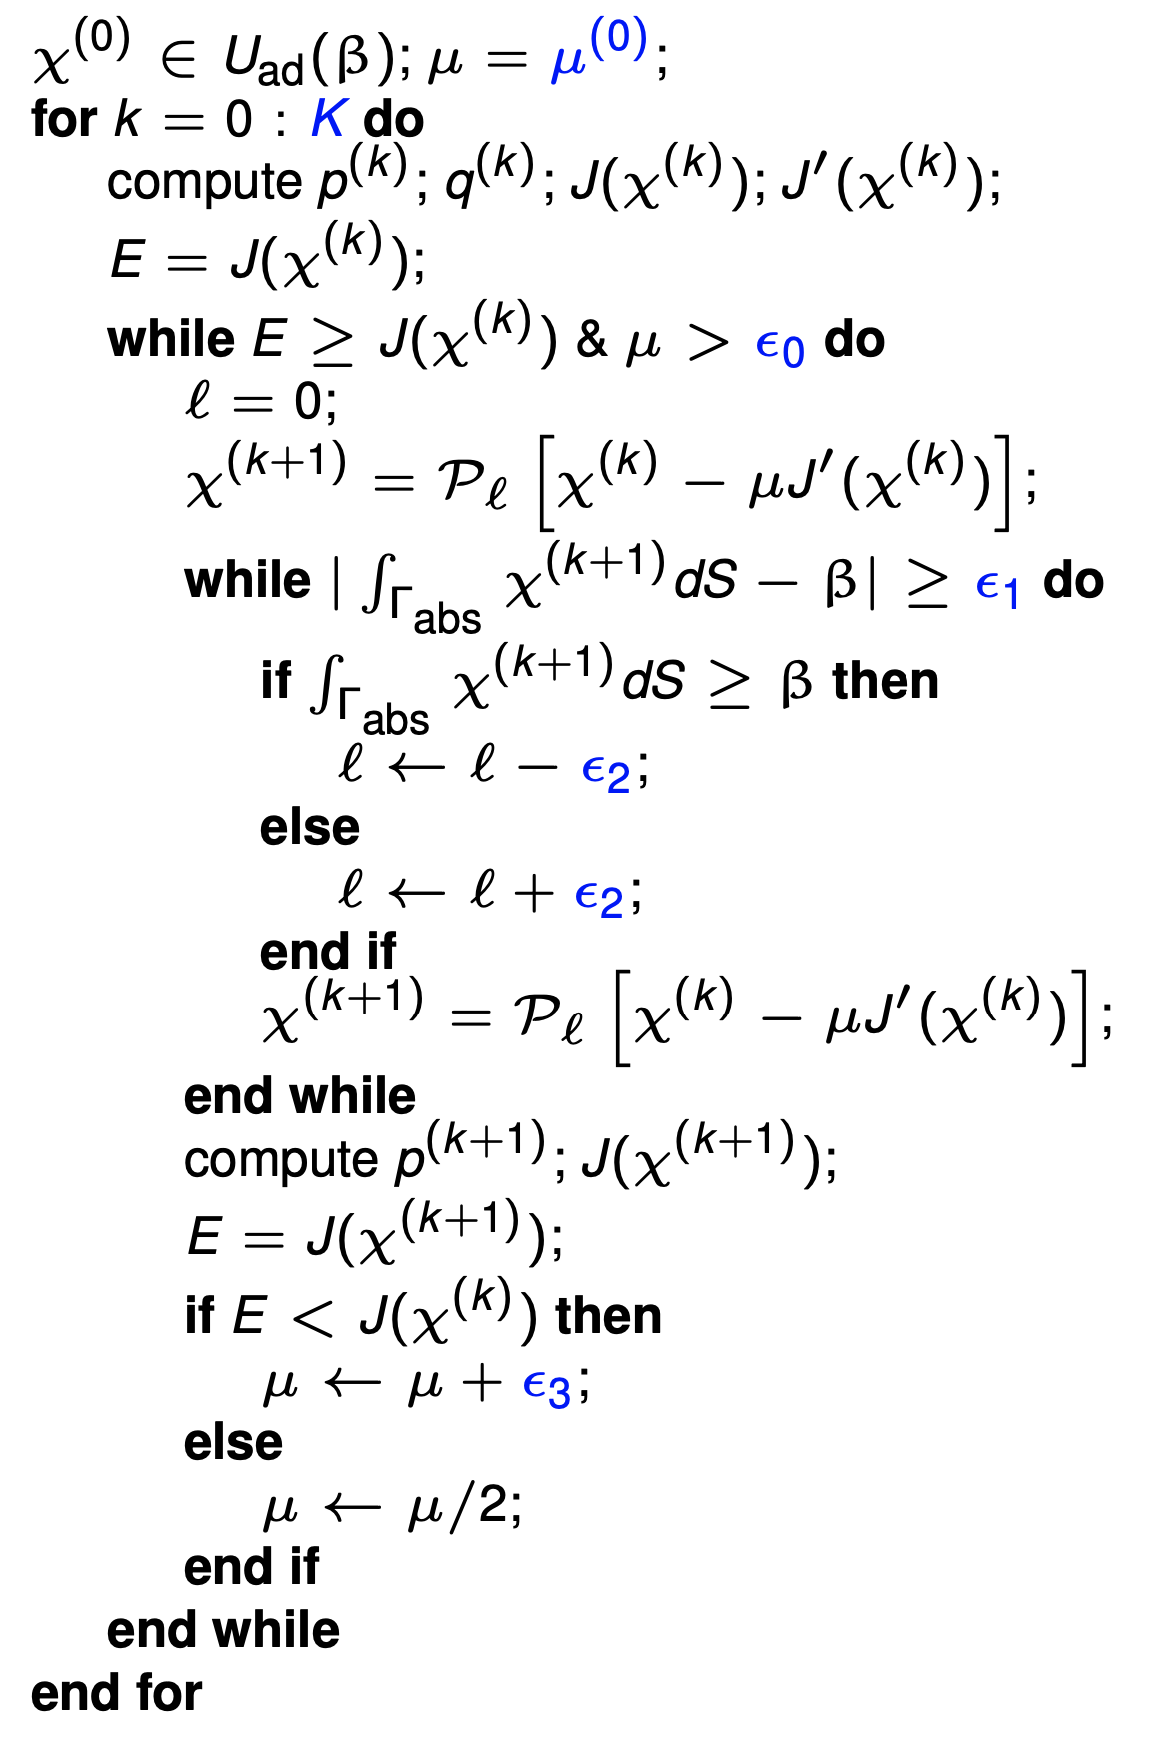
\includegraphics[width=0.3\linewidth]{rapport/numerique/assets/pseudo_code.png}
    \caption{Pseudo-code de l'algorithme du gradient appliqué à notre problème}
    \label{fig:enter-label}
\end{figure}

De ce fait, la suite $(J(\chi^{(n}))_{n \ge 0}$ va être amenée à converger théoriquement vers un minimum de $J$ car $\forall k > 0,$:
\begin{align*}
    J(\chi^{(k+1)}) - J(\chi^{(k)}) &= J(\chi^{(k)}) + \langle J'(\chi^{(k)}), -\mu_k J'(\chi^{(k)}) \rangle - J(\chi^{(k)}) + o(\mu_k J'(\chi^{(k)}))\\ 
    &= -\mu_k ||J'(\chi^{(k)})||^2 + o(\mu_k J'(\chi^{(k)})).
\end{align*}

et, avec la définition de la dérivée de Fréchet, 

\begin{equation*}
    \lim_{||\mu_k J'(\chi^{(k)})||_{\infty} \to 0} \displaystyle \frac{|o(\mu_k J'(\chi^{(k)}))|}{||\mu_k J'(\chi^{(k)})||_{\infty}} = \lim_{\mu_k \to 0} \displaystyle \frac{|o(\mu_k J'(\chi^{(k)}))|}{||\mu_k J'(\chi^{(k)})||_{\infty}} = \lim_{\mu_k \to 0} \displaystyle \frac{|o(\mu_k J'(\chi^{(k)}))|}{|\mu_k||| J'(\chi^{(k)})||_{\infty}} = \lim_{\mu_k \to 0} \displaystyle \frac{|o(\mu_k J'(\chi^{(k)}))|}{|\mu_k||| J'(\chi^{(k)})||^2_{\infty}} = 0.
\end{equation*}

D'après le polycopié de ST \cite{3}, nous avons $J'(\chi) = - \text{Re}(\alpha p_\chi q_\chi)$ où $q_\chi$ est la solution du système adjoint de $(P_\chi)$.

\begin{equation}
    \tag{$P'_\chi$}
    \begin{cases}
    \Delta q + k^2 q = -2\bar{p_\chi} \text{ dans } \Omega \\
    q = 0 \text{ sur } \Gamma_{in} \\
    \displaystyle \frac{\partial q}{\partial n} = 0 \text{ sur } \Gamma \\[5pt]
    \displaystyle \frac{\partial q}{\partial n} + \alpha \chi q = 0 \text{ sur } \Gamma_{abs}
    \end{cases}
\end{equation}

\newpage

\subsubsection{Implémentation en Python}

\begin{Python}
def your_optimization_procedure(domain_omega, spacestep, omega, f, f_dir, f_neu, f_rob, beta_pde, alpha_pde, alpha_dir, beta_neu, beta_rob, alpha_rob, Alpha, mu, chi, V_obj):
    g_dir = numpy.zeros(f_dir.shape)
    g_neu = numpy.zeros(f_neu.shape)
    g_rob = numpy.zeros(f_rob.shape)
    k = 0
    (M, N) = numpy.shape(domain_omega)
    numb_iter = 1000
    energy = numpy.zeros((numb_iter+1, 1), dtype=numpy.float64)
    
    while k < numb_iter and mu > 10**(-5):
        print('---- iteration number = ', k)
        
        # print('1. computing solution of Helmholtz problem, i.e., u')
        u = processing.solve_helmholtz(domain_omega, spacestep, omega, f, f_dir, f_neu, f_rob, beta_pde, alpha_pde, alpha_dir, beta_neu, beta_rob, alpha_rob)
        
        # print('2. computing solution of adjoint problem, i.e., p')
        q = processing.solve_helmholtz(domain_omega, spacestep, omega, -2*numpy.conjugate(u), g_dir, f_neu, f_rob, beta_pde, alpha_pde, alpha_dir, beta_neu, beta_rob, alpha_rob)
        
        # print('3. computing objective function, i.e., energy')
        energy[k] = your_compute_objective_function(domain_omega, u, spacestep)
        ene = energy[k]
        
        # print('4. computing parametric gradient')
        grad = - numpy.real(Alpha*u*q)
        number_steps = 0
        
        while ene >= energy[k] and mu > 10**(-5):
            ene_list = numpy.array([])
            mu_list = numpy.array([])
            
            # print('    a. computing gradient descent')
            new_chi = compute_gradient_descent(chi, grad, domain_omega, mu)
            
            # print('    b. computing projected gradient')
            new_chi = compute_projected(new_chi, domain_omega, V_obj)
            
            # print('    c. computing solution of Helmholtz problem, i.e., u')
            new_alpha_rob = Alpha*new_chi
            new_u = processing.solve_helmholtz(domain_omega, spacestep, omega, f, f_dir, f_neu, f_rob, beta_pde, alpha_pde, alpha_dir, beta_neu, beta_rob, new_alpha_rob)
            
            # print('    d. computing objective function, i.e., energy (E)')
            ene = your_compute_objective_function(domain_omega, new_u, spacestep)
            
            mu_list = numpy.append(mu_list, mu)
            ene_list = numpy.append(ene_list, ene)
\end{Python}
\begin{Python}    
            bool_a = ene < energy[k]
            if bool_a:
                # The step is increased if the energy decreased
                mu = mu * 1.1
            else:
                # The step is decreased is the energy increased
                mu = mu / 2
            number_steps += 1
            print("mu=" + str(mu), "ene=" + str(ene), "grad=" + str(numpy.linalg.norm(grad, numpy.infty)), "old ene=" + str(your_compute_objective_function(domain_omega, u, spacestep)))
        mu = mu_list[numpy.where(numpy.min(ene_list) == ene_list)][0]
        chi = compute_gradient_descent(chi, grad, domain_omega, mu)
        chi = compute_projected(chi, domain_omega, V_obj)
        alpha_rob = Alpha*chi
        k += 1
    energy[k] = ene
    # print('end. computing solution of Helmholtz problem, i.e., u')
    return chi, energy, u, grad
\end{Python}

\subsection{Projection de $\chi$}

Afin de restreindre $\chi^{(k+1)}$ dans $[0, 1]$ et garantir que la quantité de matériaux $\beta$ reste constante au cours des itérations, nous devons utiliser un projeteur.

\subsubsection{Calcul de $\beta$}

Premièrement, vu que $\chi$ est une fonction caractéristique, pour calculer cette quantité de matériaux numériquement,  il faut sommer toutes les valeurs de $\chi$.\\ \\
Dans le code nous travaillerons régulièrement avec la proportion de matériaux définie par $$V = \displaystyle \frac{\displaystyle \int_{\Gamma_{abs}}\chi dS}{\displaystyle \int_{\Gamma_{abs}}dS}.$$

\subsubsection{Implémentation en Python du calcul de $\beta$}

\begin{Python}
def compute_projected(chi, domain, V_obj):
    (M, N) = numpy.shape(domain)
    S = 0
    for i in range(M):
        for j in range(N):
            if domain[i, j] == _env.NODE_ROBIN:
                S = S + 1
    B = chi.copy()
    l = 0
    chi = preprocessing.set2zero(chi, domain)

    V = numpy.sum(numpy.sum(chi)) / S
\end{Python}

\subsubsection{Calcul du projecteur}

Le projecteur utilisé est $\mathcal{P}_{\ell}(\chi) = \max(0, \min(\chi + \ell, 1))$ avec $\ell$ fixé de manière à garantir $\displaystyle \int_{\Gamma_{abs}}\chi^{(k)} = \beta$. En remarquant que la fonction $\ell \mapsto \displaystyle \int_{\Gamma_{abs}}\max(0, \min(\chi + \ell, 1))dS$ est croissante, il est possible de faire une dichotomie de manière à trouver le $\ell$ correspondant à cette condition. Les bornes utilisées pour $\ell$ sont $-\max(\chi)$ et 1. Vu que,
$$\displaystyle \int_{\Gamma_{abs}}\max(0, \min(\chi - \max(\chi), 1))dS = 0 \text{ et } \displaystyle \int_{\Gamma_{abs}}\max(0, \min(\chi + 1, 1))dS = \displaystyle \int_{\Gamma_{abs}}dS,$$
cela garantit que la dichotomie va trouver un $\ell$ qui va faire converger $\displaystyle \int_{\Gamma_{abs}}\max(0, \min(\chi + \ell, 1))dS$ vers $\beta$ car $0 \le \beta \le \displaystyle \int_{\Gamma_{abs}}dS.$

\subsubsection{Implémentation en Python du projecteur (suite du code du calcul de $\beta$)}

\begin{Python}
    debut = -numpy.max(chi)
    fin = 1
    ecart = fin - debut
    # We use dichotomy to find a constant such that chi^{n+1}=max(0,min(chi^{n}+l,1)) is an element of the admissible space
    while ecart > 10**(-5):
        # calcul du milieu
        l = (debut + fin) / 2
        for i in range(M):
            for j in range(N):
                chi[i, j] = numpy.maximum(0, numpy.minimum(B[i, j] + l, 1))
        chi = preprocessing.set2zero(chi, domain)
        V = sum(sum(chi)) / S
        if V > V_obj:
            fin = l
        else:
            debut = l
        ecart = fin - debut
        # print('le volume est', V, 'le volume objectif est', V_obj)

    return chi
\end{Python}

\subsection{Problèmes rencontrés dans l'optimisation}

Quelques problèmes se sont produits avec cette première version du code.
\begin{itemize}
    \item Le programme d'optimisation s'arrêtait au bout de quelques itérations seulement à cause du critère $\mu \ge 10^{-5}$ pour rester dans la grande boucle. En effet, vu que l'algorithme n'arrive pas à trouver une valeur de $\mu_k$ pour diminuer l'énergie, le $\mu_k$ est divisé par $2$ jusqu'à être inférieur à $10^{-5}$ pour sortir de la petite boucle. Nous avons donc penser à enlever ce critère de la petite boucle et de la grande boucle, et nous l'avons remplacé par un nombre maximal d'itérations dans la petite boucle.
    \item De même, vu que le $\mu_k$ devient trop petit à cause du blocage dans la petite boucle, nous avons décidé de rajouter $10^{-3}$ à $\mu_k$ à chaque passage dans la grande boucle. Cela à une grande influence si la petite boucle s'est exécutée un trop grande nombre de fois, et ne change pratiquement rien si l'énergie a bien été diminuée au bout de quelques essais seulement.
    \item Nous avons observé que le code convergeait beaucoup plus vite et beaucoup mieux en mettant un signe "+" devant le calcul du gradient. De cette manière nous avons réalisé une bonne partie de nos tests avec ce signe "+" sans avoir plus d'explications scientifiques. Suite à cet ajout, nous avons remis le critère sur $\mu_k$ dans la petite boucle et enlevé le rajout de $10^{-3}$.
\end{itemize}

\subsection{Projection final}

\subsubsection{Explication théorique}

La dernière étape de l'algorithme est de projeter le $\chi$ optimal calculé par l'algorithme dans l'ensemble discret $\{0,1\}$ tout en conservant la quantité de matériaux $\beta$.\\ \\
Pour ce faire, nous adoptons une projection de la forme 
\begin{align*}
    \mathcal{P_\mathcal{\gamma}} 
    \colon& \mathcal{F}(\Gamma_{abs}, [0, 1]) \longrightarrow \mathcal{F}(\Gamma_{abs},\{0,1\}) \\
    &\chi \mapsto \mathbf{1}_{\chi > \gamma},
\end{align*}
où $\gamma$ est choisi de manière à avoir $\displaystyle \int_{\Gamma_{abs}} \mathcal{P_\mathcal{\gamma}} (\chi)dS = \beta$. \\ \\
Numériquement, fixer $\gamma$ revient à déterminer le nombre de points de la liste \texttt{chi} qui doivent être égaux à $1$. Nous souhaitons donc qu'il y ait exactement $\lfloor \beta \rfloor$ points dans la liste \texttt{chi} ayant la valeur $1$. (Nous utilisons la partie entière inférieure car il est préférable d'utiliser moins de matériaux que prévu plutôt que d'en utiliser trop.) Pour les sélectionner, nous choisissons simplement les $\lfloor \beta \rfloor$ points ayant les valeurs les plus élevées.

\subsubsection{Implémentation en Python}

\begin{Python}
def final_projected(chi, nb_pixels):
    # find the beta th largest value of chi
    chi_copy = chi.copy()
    chi_copy = chi_copy.reshape(-1)
    chi_copy.sort()
    chi_copy = chi_copy[::-1]
    threshold = chi_copy[nb_pixels-1]
    # set to zero all the values of chi that are smaller than the threshold
    chi[chi < threshold] = 0.
    # set to one all the values of chi that are greater than the threshold
    chi[chi >= threshold] = 1.
    return chi
\end{Python}

\newpage

\section{Analyse des résulats}
\subsection{Un premier résultat préliminaire}
On teste l'algorithme de descente de gradient pour un nombre d'onde $k=1$ et un mur de fractale de niveau 2.
La Figure \ref{fig:ene1} représente l'évolution de l'énergie (ou la fonction coût) en fonction du nombre d'itérations lors de l'application de l'algorithme d'optimisation par descente de gradient. Le nouveau $\chi$ calculé par l'algorithme permet de diminuer l'énergie au sein du réacteur.

\begin{figure}[H]
    \centering
    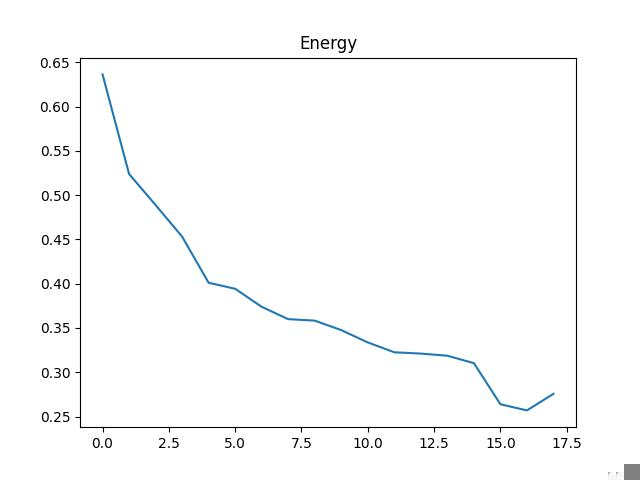
\includegraphics[width=0.5\linewidth]{rapport//numerique//exemplek1/k0descgradenergy.jpg}
    \caption{Énergie en fonction du nombre d'itération}
    \label{fig:ene1}
\end{figure}



\begin{figure}[H]
    \centering
    \subfloat{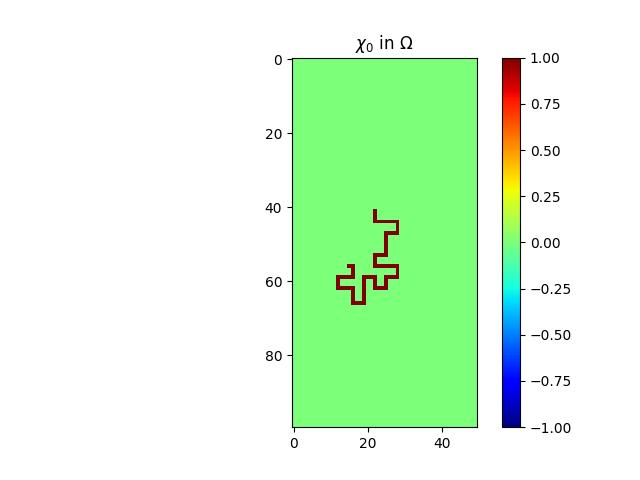
\includegraphics[width = 3.0in]{rapport/numerique/exemplek1/fig_chi0_re_plot_k1.jpg}
    \subfloat{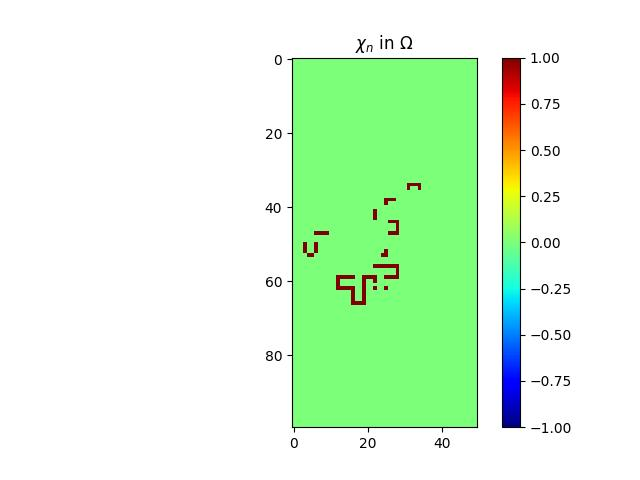
\includegraphics[width = 3.0in]{rapport/numerique/exemplek1/fig_chin_re_plot_k1.jpg}}\\
    \caption{$\chi$ avant et après optimisation et projection}
    \label{loca}
\end{figure}

\begin{figure}[H]
    \centering
    \subfloat{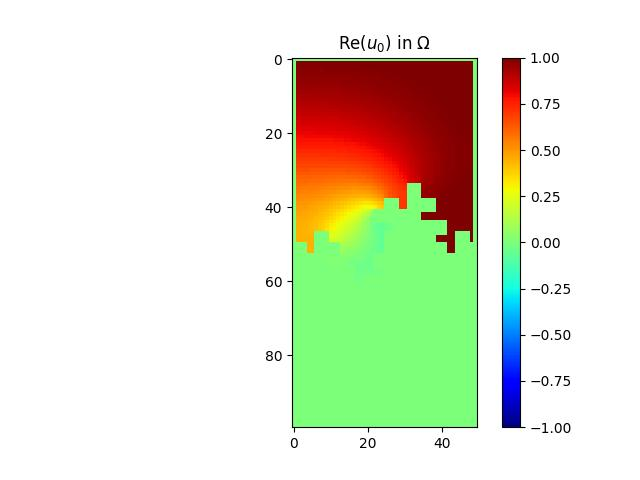
\includegraphics[width = 3.0in]{rapport/numerique/exemplek1/fig_u0_re_plot.jpg}}
    \subfloat{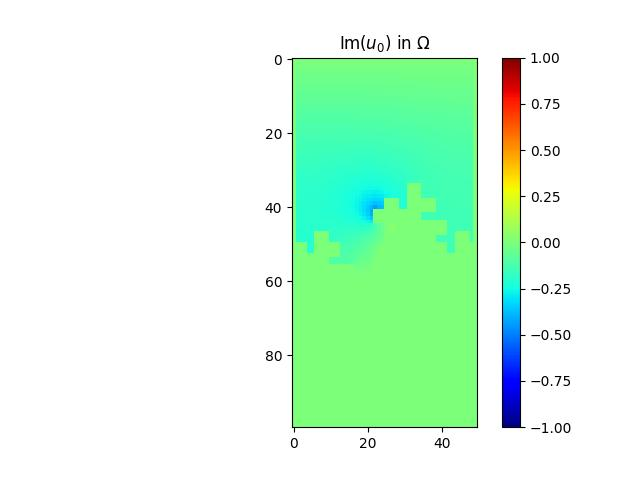
\includegraphics[width = 3.0in]{rapport/numerique/exemplek1/fig_u0_im_plot.jpg}}\\
    \caption{Solution $u$ avant optimisation}
    \label{loca}
\end{figure}

\begin{figure}[H]
    \centering
    \subfloat{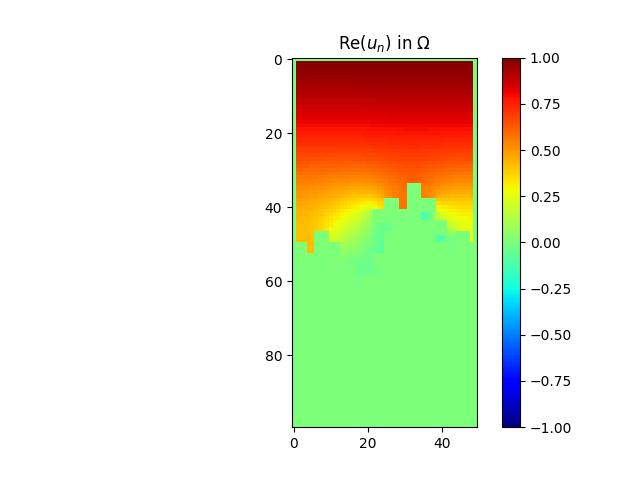
\includegraphics[width = 3.0in]{rapport/numerique/exemplek1/fig_un_re_plot.jpg}}
    \subfloat{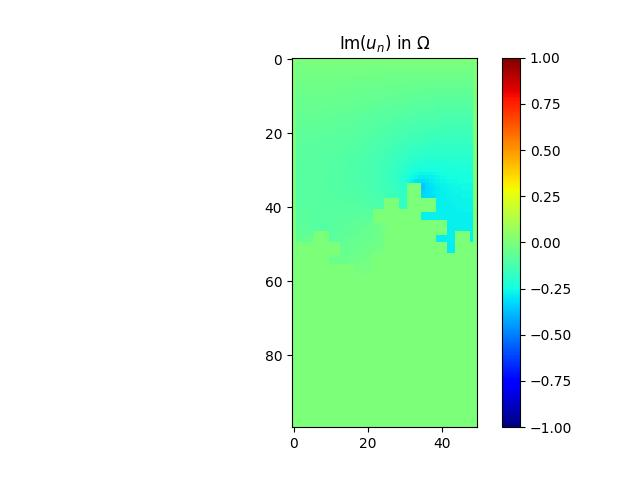
\includegraphics[width = 3.0in]{rapport/numerique/exemplek1/fig_un_im_plot.jpg}}\\
    \caption{Solution $u$ après optimisation}
    \label{loca}
\end{figure}


\subsection{Étude des bruits}
Pour que l'atténuation du bruit de l'avion soit efficace, il est nécessaire d'étudier la fréquence des bruits qui dérangent le plus. Les bruits crées par les moteurs d'avion proviennent de trois sources principalement: le ventilateur, la turbine et la combustion. La combinaison de ces bruits se situe généralement entre 100 Hz et 6 000 Hz. Étant donné que $ k = \omega/c = 2\pi f/c$, nous allons donc étudier le problème pour $k \in [1.85\,m^{-1}, 112\,m^{-1}].$ 

\subsection{Étude des matériaux}
Dans cette section, on fera une étude comparative entre différents matériaux qui peuvent être utilisés dans la fabrication des liners en termes de qualité d'absorption de l'énergie sonore que nous cherchons à minimiser. En effet, la qualité d'absorption du matériau dépend du coefficient $\alpha$ qui dépend lui même aussi de la fréquence utilisée. Comme il est nécessaire d'utiliser un matériau léger, résistant et poreux, nous avons choisi de comparer trois matériaux: l'Isorel, l'IFTH, et le mat q3. Ces matériaux ont 3 grandeurs caractéristiques qui affectent leur capacité d'absorbance, à savoir la porosité $\phi$, la résistivité $\sigma$ et la tortuosité $\alpha_{h}$, montrés dans le tableau suivant.
\begin{table}[H]
\centering
\begin{tabular}{|c|c|c|c|c|}
\hline
Caractéristique & mat q3 & IFTH  & Isorel \\ \hline
$\phi$ & 0.99 & 0.94 & 0.70 \\ \hline
$\sigma$ & 14000 & 9067 & 142300 \\ \hline
$\alpha_{h}$ & 1.02 & 1 & 1.15 \\ \hline
\end{tabular}
\caption{Caractéristiques des différentes matériaux}
\end{table}
Nous avons donc évalué le coefficient $\alpha$ de ces différents matériaux sur une plage de fréquences entre 50Hz et 1kHz. Les résultats de simulation sont les suivants.

\begin{figure}[H]
    \centering

    \subfloat{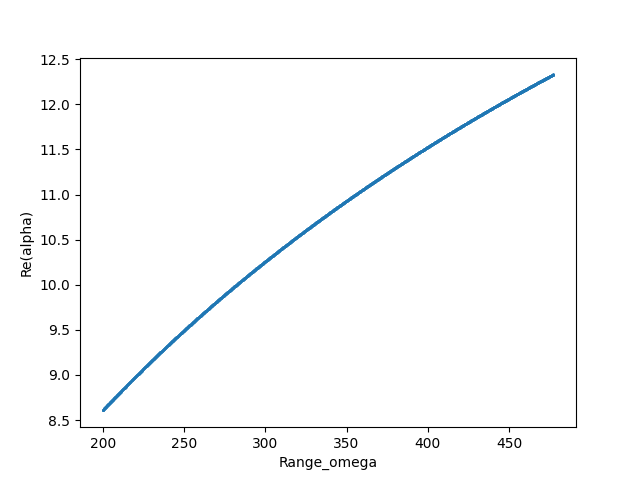
\includegraphics[width = 3.0in]{rapport/numerique/Re(alpha) mat q3.png}
    \subfloat{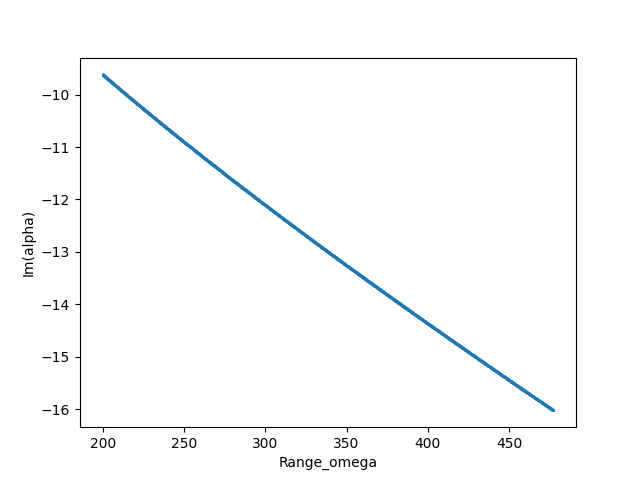
\includegraphics[width = 3.0in]{rapport/numerique/Im(alpha) mat q3.png}}\\
    \caption{$Re(\alpha)$ et $Im(\alpha)$ pour mat q3}
    \label{freq}
\end{figure}

\begin{figure}[H]
    \centering

    \subfloat{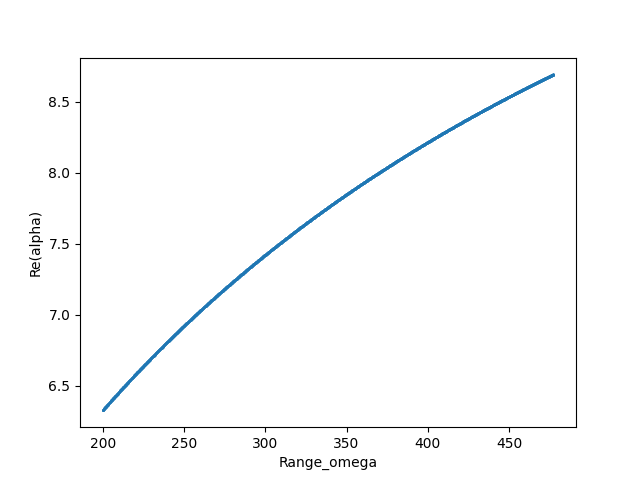
\includegraphics[width = 3.0in]{rapport/numerique/Re(alpha) ITFH.png}
    \subfloat{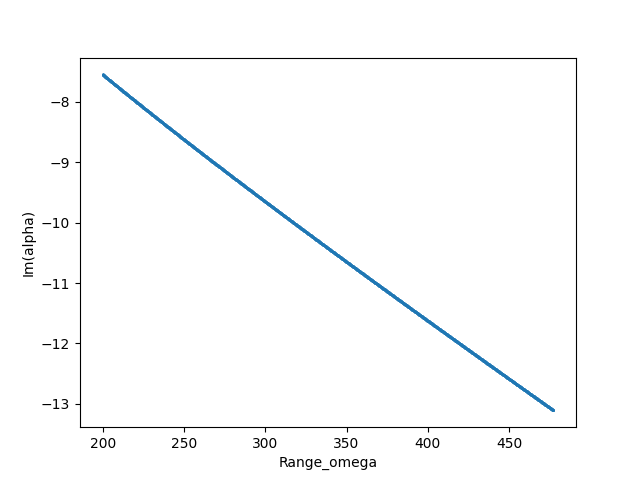
\includegraphics[width = 3.0in]{rapport/numerique/Im(alpha) ITFH.png}}\\
    \caption{$Re(\alpha)$ et $Im(\alpha)$ pour ITFH}
    \label{freq}
\end{figure}

\begin{figure}[H]
    \centering

    \subfloat{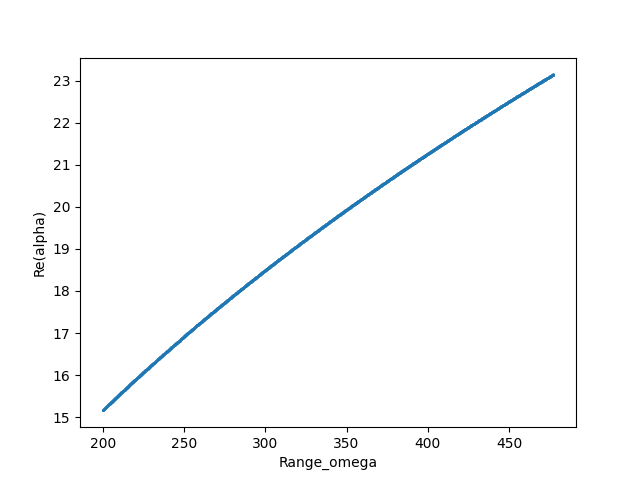
\includegraphics[width = 3.0in]{rapport/numerique/Re(alpha) isorel.png}
    \subfloat{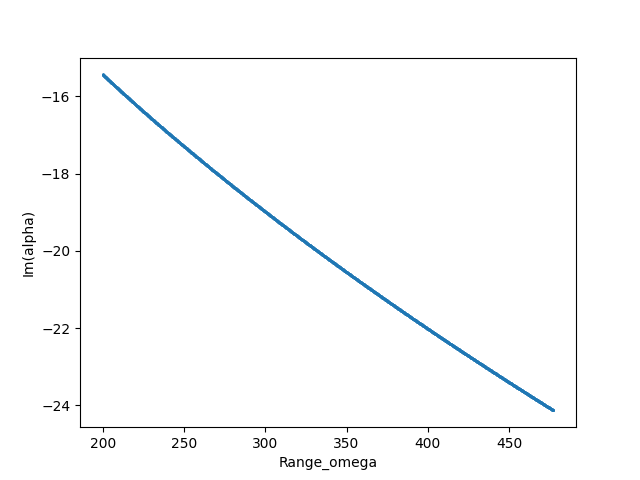
\includegraphics[width = 3.0in]{rapport/numerique/Im(alpha) ISOREL.png}}\\
    \caption{$Re(\alpha)$ et $Im(\alpha)$ pour ISOREL}
    \label{freq}
\end{figure}

La compréhension des courbes passe par l'évolution de la partie réelle et imaginaire de $\alpha$. En effet, plus le rapport de $\displaystyle \frac{Re(\alpha)}{Im(\alpha)}$
est proche de 0 plus le matériau est absorbant.
\begin{figure}[H]
    \centering
    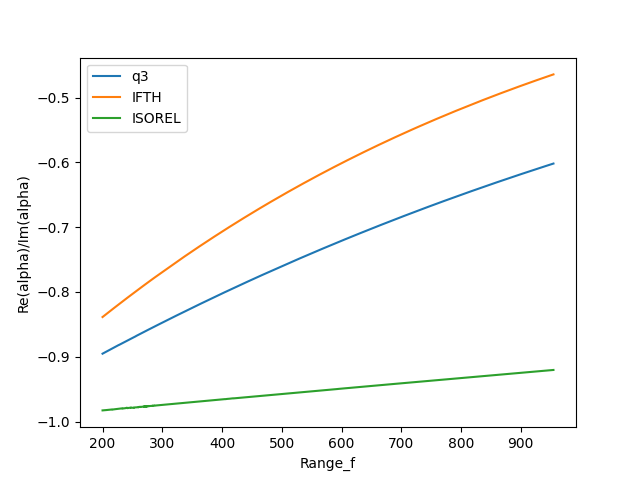
\includegraphics[width=0.5\linewidth]{rapport/numerique/Re(alpha) over Im(alpha)_ISOREL.png}
    \caption{$\displaystyle \frac{Re(\alpha)}{Im(\alpha)}$ pour les 3 matériaux}
    \label{fig:ene}
\end{figure}

La figure nous montre que c'est l'IFTH le matériau le plus absorbant parmi les 3 et c'est celui qu'il faut adopter pour la construction du matériau poreux au niveau de la frontière de bas.\\
Cependant, pour les sections qui suivent, nous utiliserons un coefficient $\alpha$ de $10-10j$ assez souvent afin de s'approcher de l'ordre de grandeur général des parties réelles et imaginaires de $\alpha$ trouvées pour les différents matériaux étudiés.

\subsection{Étude de la géométrie}
Dans cette section, nous étudions l'énergie au sein du réacteur en fonction de la géométrie de la frontière afin de déterminer la géométrie la plus efficace. Pour cette étude, la frontière est totalement absorbante (\textit{id est} \\ $V = \displaystyle \frac{\int_{\Gamma_{abs}} \chi dS}{\int_{\Gamma_{abs}} dS} = 1$), et on trace l'énergie sur toute la gamme de fréquence considérée pour chaque niveau de fractale.
\begin{figure}[H]
    \centering
    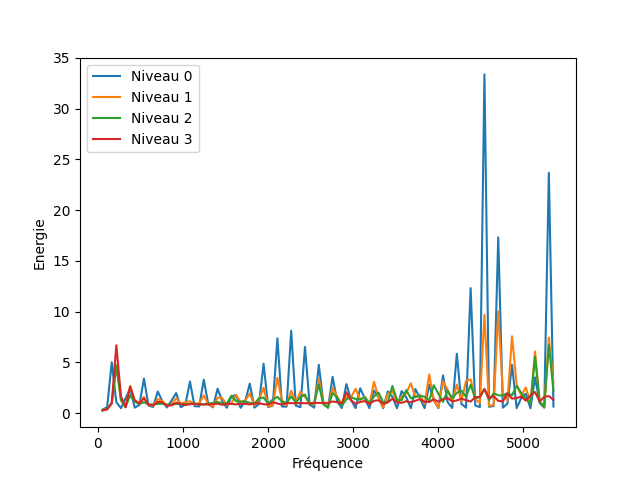
\includegraphics[width=0.5\linewidth]{rapport/numerique/exemplek1/fullabs.png}
    \caption{Frontière totalement absorbante pour différents niveaux de fractale}
    \label{fig:enter-label}
\end{figure}
Nous obtenons le tableau suivant.
\begin{table}[H]
    \centering
    \begin{tabular}{ccc}
        Fractale & Énergie Max  & Énergie Moyenne\\
         Niveau 0& 33,4 & 2,45 & \\
         Niveau 1 & 10,0 & 1,88 & \\
         Niveau 2 & 6,74 & 1,51 & \\
         Niveau 3 & 6,70 & 1,20 & \\
    \end{tabular}
    \label{tab:my_label}
\end{table}
Ainsi une fractale de niveau 2 et de niveau 3 atténue bien mieux les bruits. Dans la suite de l'étude, nous ne considérons seulement ces deux niveaux de fractale.\\ \\
Cependant, une remarque doit être vis-à-vis des différents niveaux de fractale choisis. Plus le niveau de fractale est élevé, plus la longueur de la paroi est grande et plus la quantité de matériaux nécessaire augmente. Le choix de conserver les niveaux 2 et 3 seulement s'explique par le fait que nous voulons une solution de bonne qualité, même si cela nécessite plus de matériaux. Néanmoins, il se peut que nous privilégions le niveau 2 au 3 car le niveau 3 n'apporte pas suffisamment de réduction par rapport au niveau 2.

\subsection{Étude de la quantité de matériaux}
On étudie l'efficacité de l'atténuation en fonction de la quantité de matériaux utilisé par le liner afin de trouver le meilleur compromis entre atténuation et coût.
    \begin{figure}[H]
    \centering
    \subfloat{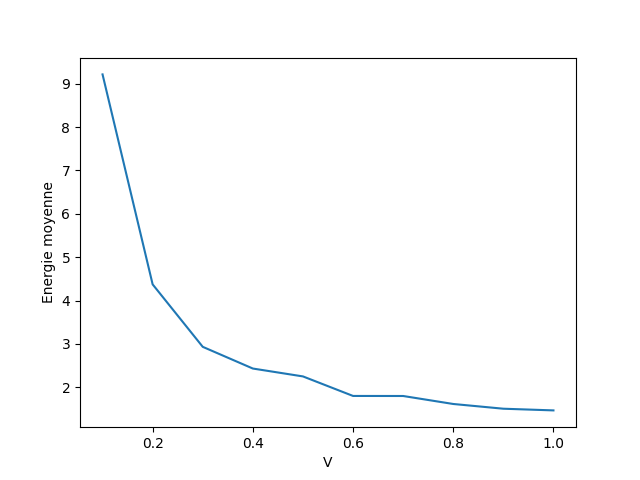
\includegraphics[width = 3.0in]{rapport/numerique/exemplek1/lvl2.png}}
    \subfloat{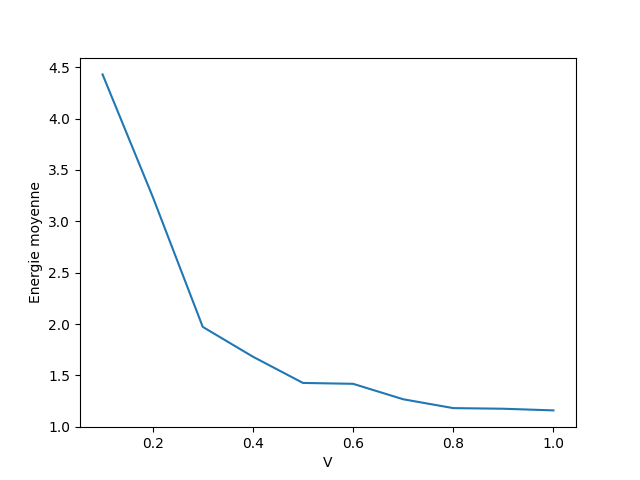
\includegraphics[width = 3.0in]{rapport/numerique/assets/lvl3.png}}\\
    \caption{Énergie moyenne après optimisation en fonction de $V$ pour la fractale de niveau 2 (gauche) et 3 (droite)}
    \label{freq}
\end{figure}

\subsection{Optimisation mono-fréquentielle}

Dans cette section, nous allons optimiser la disposition du liner pour atténuer les fréquences les plus problématiques. Pour chaque niveau de fractale, on choisit les 7 fréquences pour lesquelles les énergies sont les plus grandes. La Figure \ref{freq1} montre que pour toutes ces fréquences problématiques, l'énergie après optimisation diminue largement. Notre algorithme permet donc d'atténuer les fréquences problématiques.

\begin{figure}[H]
    \centering
    \subfloat{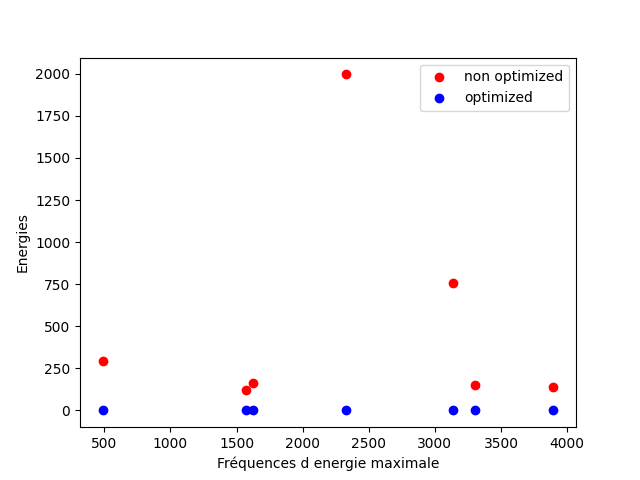
\includegraphics[width = 3.0in]{rapport/numerique/assets/Level_2_Alpha_absorp_N_50.png}}
    \subfloat{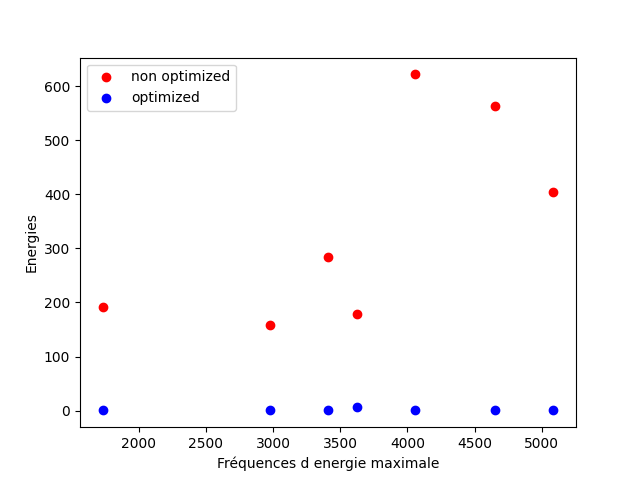
\includegraphics[width = 3.0in]{rapport/numerique/assets/Level_3_Alpha_absorp_N_50.png}}\\
    \caption{Les énergies maximales en fonction de la fréquence pour une fractale de niveau 2 et 3}
    \label{freq1}
\end{figure}

\subsection{Optimisation multi-fréquentielle}
La section précédente montre que notre algorithme est efficace pour chacune des fréquences considérées comme problématique, nous cherchons maintenant à étudier s'il est possible d'optimiser pour l'ensemble de ces fréquences simultanément. Nous devons alors adapter notre algorithme de descente de gradient. 

En effet, la nouvelle fonction de coût à considérer est la somme des énergies des fréquences pour un même $\chi$ pondérées avec des réels $(\lambda_{k})_{k \in K}$ (nous avons pris l'énergie avant: \textcolor{blue}{$$J(\chi) := \sum_{k} \lambda_{k} \int_\Omega |p_{k_{\chi}}|^2$$} et le gradient à considérer est alors la somme des gradients de chaque fréquence pondérée : \textcolor{blue}{$$J'(\chi) := - \sum_{k} \lambda_{k} \text{Re}(\alpha p_{k} q_{k}).$$}

En cherchant à minimiser la fonction de coût, l'algorithme va donner $\chi $ qui minimise globalement pour l'ensemble des fréquences considérées. Pour le choix des coefficients de pondération $\lambda_{k}$, nous avons pris l'énergie pour une onde de nombre de d'onde $k$ avant optimisation. 
Cependant, ce nouveau algorithme effectue beaucoup plus de calcul, c'est pourquoi nous nous limitons aux dix premiers $k$ en énergie pour avoir un temps de calcul raisonnable. Nous avons aussi limiter un nombre d'itération maximale à 10.

\begin{figure}[H]
    \centering
    \subfloat{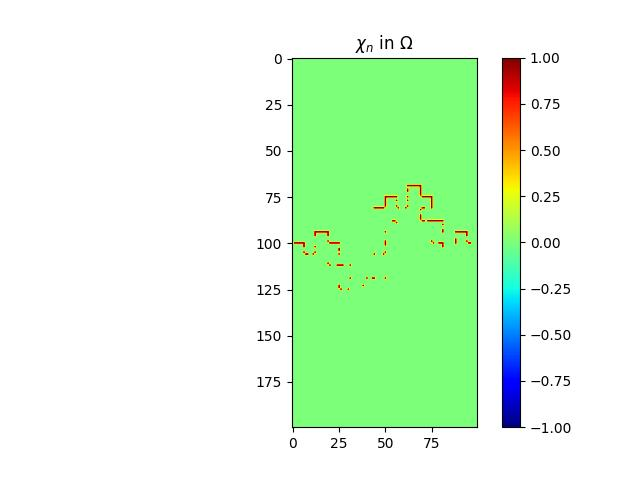
\includegraphics[width = 3.0in]{rapport/numerique/exemplek1/chimulti2.jpg}}
    \subfloat{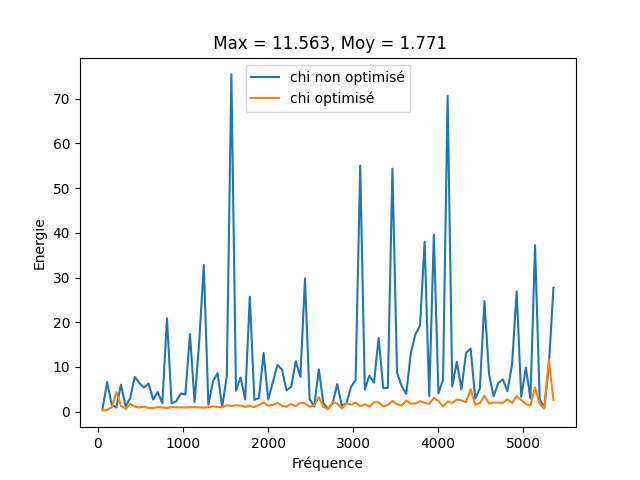
\includegraphics[width = 3.0in]{rapport/numerique/exemplek1/multi2.png}}\\
    \caption{Optimisation multi-fréquentielle avec fractale de niveau 2}
    \label{freq}
\end{figure}
\begin{figure}[H]
    \centering
    \subfloat{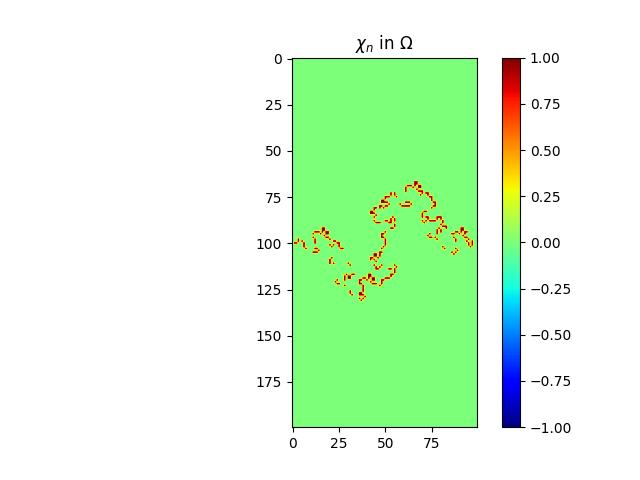
\includegraphics[width = 3.0in]{rapport/numerique/exemplek1/chimulti3.jpg}
    \subfloat{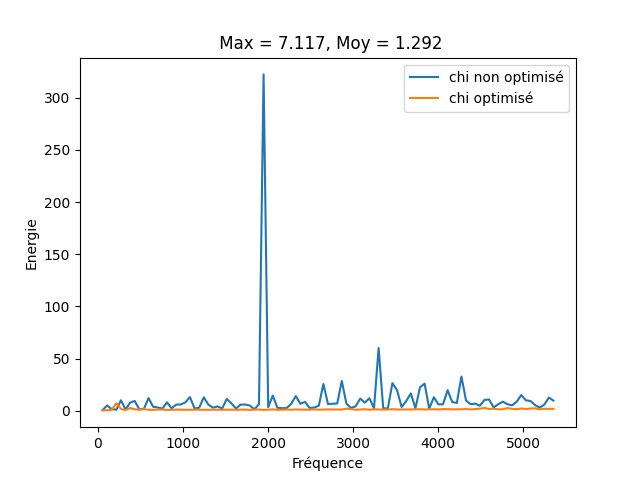
\includegraphics[width = 3.0in]{rapport/numerique/exemplek1/multi3.png}}\\
    \caption{Optimisation multi-fréquentielle avec fractale de niveau 3}
    \label{freq}
\end{figure}
Les figures obtenues montrent que l'optimisation multi-fréquentielle est très efficace: après optimisation, pour les niveaux de fractale, l'énergie est relativement faible sur toute la gamme de fréquence.

\subsection{Autre approche : optimisation stochastique}
On se propose d'étudier ce problème d'optimisation en utilisant une autre méthode que l'algorithme de descente gradient, plus particulièrement l'algorithme d'optimisation stochastique Hill Climbing. On commence par générer $\chi$ aléatoirement. A chaque itération, on explore le voisinage de $\chi$ en ajoutant un bruit blanc à $\chi$. Si avec le $\chi$ bruité l'énergie diminue, alors l'ancien $\chi$ est remplacé par le $\chi$ bruité, puis on itère un certain nombre de fois.
Expérimentalement on observe qu'entre le début et la fin de l'algorithme, la différence d'énergie est minimale. C'est pourquoi on limite à une seule itération, ce qui revient à utiliser un $\chi$ aléatoire.

\begin{figure}[H]
    \centering
    \subfloat{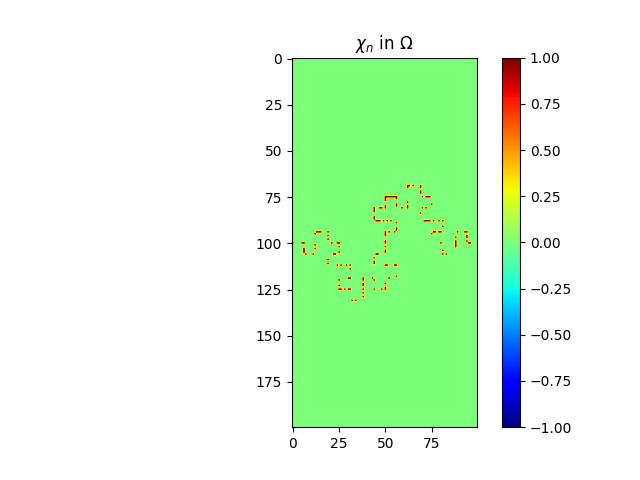
\includegraphics[width = 3.0in]{rapport/numerique/assets/rand/chi_rand_2.jpg}}
    \subfloat{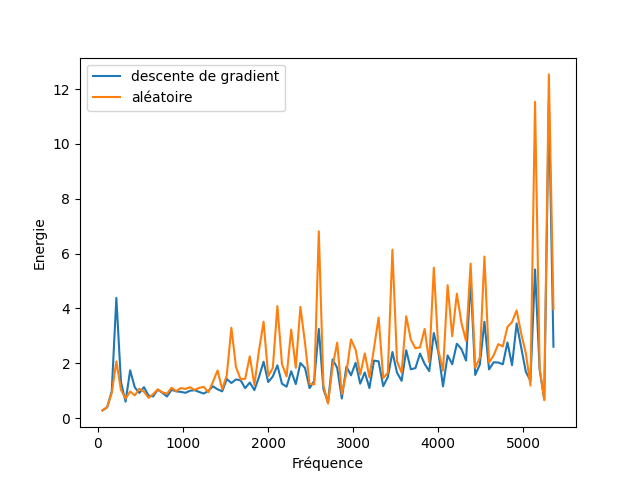
\includegraphics[width = 3.0in]{rapport/numerique/exemplek1/vslvl2.png}}\\
    \caption{Optimisation stochastique avec fractale de niveau 2}
    \label{vs1}
\end{figure}
\begin{figure}[H]
    \centering
    \subfloat{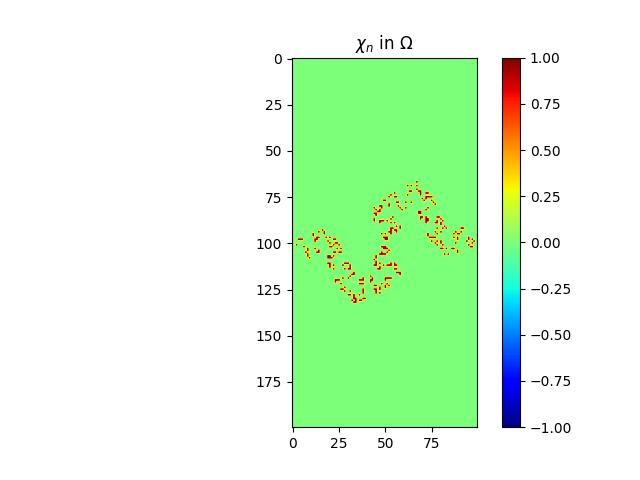
\includegraphics[width = 3.0in]{rapport/numerique/exemplek1/chi_rand_3.jpg}
    \subfloat{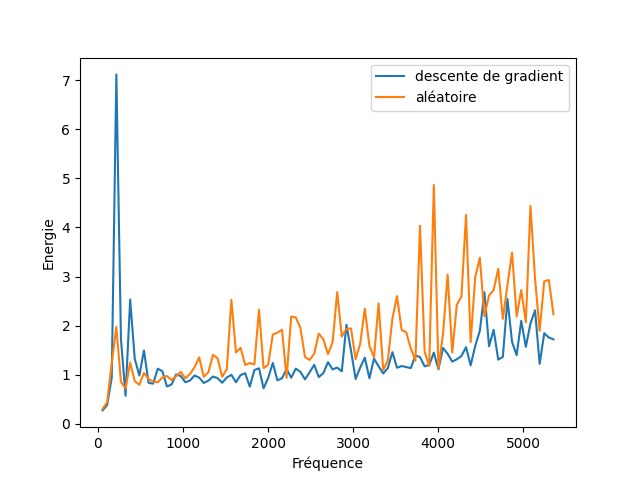
\includegraphics[width = 3.0in]{rapport/numerique/exemplek1/vslvl3.png}}\\
    \caption{Optimisation stochastique avec fractale de niveau 3}
    \label{vs2}
\end{figure}

D'après les Figures \ref{vs1} et \ref{vs2}, on conclut que l'optimisation stochastique est légèrement moins efficace que l'algorithme de descente de gradient multi-fréquentielle. Cependant, elle est également beaucoup plus rapide à calculer. De plus, on peut remarquer que pour la fractale de niveau 3, pour une fréquence particulière, l'énergie de la solution donnée par l'algorithme de descente de gradient est bien plus élevée que celle du $\chi$ aléatoire. \\ \\
Le caractère aléatoire de cette méthode d'optimisation va permettre d'avoir un $\chi$ qui est généralement réparti plutôt uniformément sur toute la paroi du réacteur, d'où l'atténuation efficace.

\subsection{Solution retenue}

D'après l'ensemble des études effectuées, la solution retenue est une fractale de niveau 2, $V = 0,5$, optimisé avec l'algorithme de descente de gradient multi-fréquentielle. On peut comparer son efficacité avec une fractale de niveau 3 entièrement absorbant dans la Figure \ref{abs22}.
\begin{figure}[H]
    \centering
    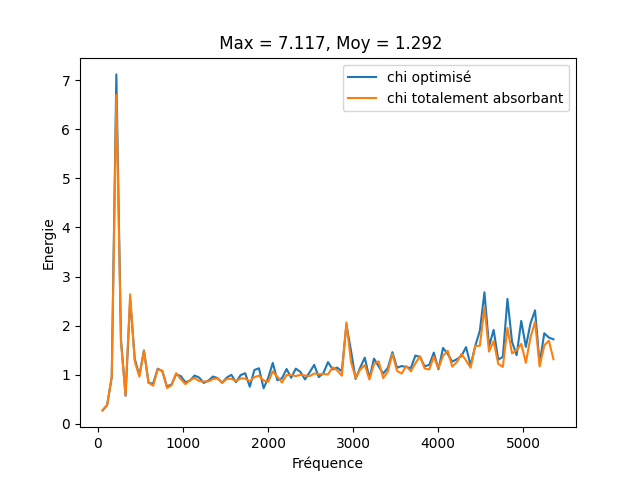
\includegraphics[width=0.5\linewidth]{rapport/numerique/exemplek1/solvsfullabs.png}
    \caption{Comparaison entre notre solution optimisée et $\chi$ totalement absorbant}
    \label{abs22}
\end{figure}
On peut remarquer la performance de la solution optimisée est très proche de $\chi$ totalement absorbant, voire meilleure pour certaines fréquences, alors qu'on utilise beaucoup moins de matériau absorbant ! 

\subsection{Conclusion de la partie numérique}
En résumé, notre démarche pour résoudre le problème posé est la suivante :
    \begin{itemize}
        \item Implémentation d'un algorithme de descente de gradient;
        \item Plusieurs études pour choisir des paramètres adaptés;
        \item Détermination de la meilleure solution en tenant en compte des études précédentes.
    \end{itemize}
Nous envisageons également quelques pistes d'amélioration possibles: 
    \begin{itemize}
        \item Meilleur ajustement des hyperparamètres (comme le learning rate) ;
        \item Mise à jour dynamique des coefficients de pondération pendant l'algorithme de descente de gradient multi-fréquentielle. En effet, les fréquences problématiques peuvent changer lorsque $\chi$ est modifié ;
        \item Calculer la réduction de bruit réelle en décibel ;
        \item Explorer d'autres algorithmes d'optimisation, comme l'algorithme génétique par exemple.
    \end{itemize}
\end{frame}

\newpage

\section{Etude du problème variationnel}
\begin{tcolorbox}[colback=blue!5!white,colframe=blue!75!black,title=Definition 4.0: Problème différentiel]
On souhaite résoudre le problème différentiel suivant d'un point de vue théorique:

\[
    (P) \hspace{2pt} : \hspace{2pt}
    \begin{cases}
    \displaystyle \Delta p + k_0^2\Big(1 - \frac{iM_0}{k_0}\frac{\partial}{\partial x}\Big)^2p = f \in L^2(\Omega) \hfill (i)\\
    \displaystyle Z\frac{\partial p}{\partial n} + ik_0Z_0\chi \Tr \Bigl[ \Bigl(1-i \frac{M_0}{k_0} \Big(\frac{\partial}{\partial x} + \frac{\partial}{\partial y}\Big) \Bigr)^2p \Bigr] = 0$ sur $\Gamma = \Gamma_1 \sqcup \Gamma_2 \hspace*{2cm} \hfill (ii)
    \\
    \displaystyle \Tr(p) = g $ sur $ \Gamma_{in} \hfill (iii) \\
    \displaystyle \frac{\partial p}{\partial n} + ik \Tr(p) = 0 $ sur $\Gamma_{out} \hfill (iv)
    \end{cases} 
\]

avec : $\displaystyle Z_0 \in \mathbb{R}$,  $Z \in \{z \in \mathbb{C} \hspace{2pt} | \hspace{2pt} Re(z) > 0\}$, $\chi : \Gamma \to \{0,1\} $, $\displaystyle M_0 = \frac{u_0}{c_0}$, $\displaystyle k_0 = \frac{\omega}{c_0}$, $\displaystyle k = \frac{\omega}{u_0}$.

$M_0$ dit "Nombre de Mach" est le rapport entre la vitesse du fluide et la célérité d'une onde acoustique, $k_0$ est le "nombre d'onde acoustique" et $k$ est le "nombre d'onde fluide".

On rappelle également que $\partial \Omega = \Gamma \sqcup \Gamma_{in} \sqcup \Gamma_{out}$. \\
On n'oubliera pas que $\Omega$ peut être à bord localement lipschitzien tout comme à bord fractal, donc  $\partial \Omega$ n'est pas nécessairement régi par la mesure de Lebesgue. On appelera donc $\mu$ la mesure choisie sur le bord.

\end{tcolorbox}

\subsection{Formulation variationnelle}

Notre objectif sera de trouver le problème variationnel équivalent que l'on résoudra sur un espace de Hilbert $V(\Omega)\subset H^1(\Omega)$, pour l'instant indéterminé. \\

Un premier problème que l'on rencontre est, lors de l'application de la formule de Green pour trouver le problème variationnel, l'apparition d'un terme $\displaystyle \int_{\Gamma_{in}} \frac{\partial p}{\partial n} \Tr(\Bar{q})\hspace{2pt} d\mu$, qui ne peut pas s'exprimer en fonction de $g$ sur $\Gamma_{in}$. \\

Pour y remédier, on applique une méthode dite de "translation" :

\begin{tcolorbox}[colback=red!5!white,colframe=red!75!black,title=Proposition 4.1.1: Problème différentiel homogène]
n considère $p_s = p_h + p_g$ tel que $p_s$ soit solution du problème originel et $p_g\in H^1(\Omega)$ un "paramètre" qui vérifie $(ii),(iii)$ et $(iv)$. $p_h$ vérifie alors l'équation homogène associée :\\

\[
    (P_H) \hspace{2pt} : \hspace{2pt}
    \begin{cases}
    \displaystyle \Delta p + k_0^2\Big(1 - \frac{iM_0}{k_0}\frac{\partial}{\partial x}\Big)^2p = \Tilde{f} \in L^2(\Omega) \hfill (i')\\
    \displaystyle Z\frac{\partial p}{\partial n} + ik_0Z_0\chi \Tr \Bigl[ \Bigl(1-i \frac{M_0}{k_0} \Big(\frac{\partial}{\partial x} + \frac{\partial}{\partial y}\Big) \Bigr)^2p \Bigr] = 0$ sur $\Gamma = \Gamma_1 \sqcup \Gamma_2 \hspace*{2cm} \hfill (ii')
    \\
    \displaystyle \Tr(p) = 0 $ sur $ \Gamma_{in} \hfill (iii') \\
    \displaystyle \frac{\partial p}{\partial n} + ik \Tr(p) = 0 $ sur $\Gamma_{out} \hfill (iv')
    \end{cases} 
\]
où \[
    \displaystyle \Tilde{f} = f - \Delta p_g - k_0^2\Big(1 - \frac{iM_0}{k_0}\frac{\partial}{\partial x}\Big)^2p_g\]
\end{tcolorbox}
Il suffit de s'assurer que $p_g$ soit assez régulière de sorte que $\Tilde{f}\in L^2(\Omega)$.

On s'intéresse alors uniquement au problème homogène dans ce rapport. Soit $q\in V(\Omega)$ une fonction test de notre espace de Hilbert et $p$ solution de $(P_H)$ :

\begin{equation}
    (i') \Longrightarrow -\int_{\Omega} \Delta p \hspace{2pt} \overline{q}\hspace{2pt} d\lambda -k_0^2 \int_{\Omega} pq\hspace{2pt} d\lambda +2iM_0 k_0\int_{\Omega} \frac{\partial p}{\partial x}\overline{q} d\lambda +M_0 ^2 \int_{\Omega} \frac{\partial^2 p}{\partial x^2} \overline{q}\hspace{2pt} d\lambda = -\int_{\Omega} \Tilde{f}\overline{q}\hspace{2pt} d\lambda
\end{equation}

On a d'une part, d'après la formule de Green :

\begin{equation}
    \int_{\Omega} \Delta p\hspace{2pt} \overline{q}\hspace{2pt} d\lambda=-\int_{\Omega} \nabla p \nabla \overline{q}\hspace{2pt} d\lambda + \int_{\partial \Omega} \frac{\partial p}{\partial n} \Tr(\overline{q}) \hspace{2pt} d\mu
\end{equation}


\begin{equation}
    \int_{\Omega} \frac{\partial^2 p}{\partial x^2}\overline{q} d\lambda = -\int_{\Omega} \frac{\partial p}{\partial x} \frac{\partial \overline{q}}{\partial x}d\lambda + \int_{\partial \Omega} \frac{\partial p}{\partial x} \cdot n_x \Tr(\overline{q})\hspace{2pt} d\mu
\end{equation}



Etudions l'intégrale sur le bord :

\begin{equation}
    \int_{\partial \Omega} \frac{\partial p}{\partial n} \Tr(\overline{q}) \hspace{2pt} d\mu = 
    -i k \int_{\Gamma_{out}} \Tr(p) \Tr(\overline{q})\hspace{2pt} d\mu \underbrace{-ik_0 \frac{Z_0}{Z}\int_{\Gamma} \Tr \Bigl[ \Bigl(1-i \frac{M_0}{k_0} \Big(\frac{\partial}{\partial x} + \frac{\partial}{\partial y}\Big) \Bigr)^2p \Bigr] \Tr(\overline{q}) \hspace{2pt} \chi \hspace{2pt} d\mu}_{:= \hspace{2pt} C}
\end{equation}



Où l'intégrale nommée $C$ vaut:

\begin{equation}
    C = -ik_0\frac{Z_0}{Z} \biggl[ \int_{\Gamma} \Tr(p) \Tr(\overline{q}) \hspace{2pt} \chi \hspace{2pt} d\mu - 2i\frac{M_0}{k_0} \int_{\Gamma} \Tr \Bigl( \frac{\partial p}{\partial x}+\frac{\partial p}{\partial y} \Bigr) \Tr(\overline{q}) \hspace{2pt} \chi \hspace{2pt} d\mu - \frac{M_0^2}{k_0^2} \int_{\Gamma} \Tr \Bigl( \frac{\partial^2 p}{\partial x^2}+2\frac{\partial^2 p}{\partial x \partial y} + \frac{\partial^2 p}{\partial y^2} \Bigr)\Tr(\overline{q}) \hspace{2pt} \chi  \hspace{2pt} d\mu \biggl]
\end{equation}
On peut supposer que la condition au bord est définie presque partout ; en prenant donc cette condition égale à 0 sur le "bord du bord", et en supposant en outre qu'on puisse permuter la dérivée et l'opérateur de trace, cela nous donne :



\begin{equation} \displaystyle
    \begin{cases}
    \displaystyle \int_{\Gamma} \Tr \Bigr(\frac{\partial^2 p}{\partial x^2}\Bigl) \Tr(\overline{q}) \chi \hspace{2pt} d\mu = - \int_{\Gamma} \Tr \Bigl( \frac{\partial p}{\partial x} \Bigr) \Tr \Bigl( \frac{\partial \overline{q}}{\partial x}\Bigr)\chi d\mu \\

    \displaystyle \int_{\Gamma} \Tr \Bigr(\frac{\partial^2 p}{\partial y^2}\Bigl) \Tr(\overline{q})\chi \hspace{2pt} d\mu = - \int_{\Gamma} \Tr \Bigl( \frac{\partial p}{\partial y} \Bigr) \Tr \Bigl( \frac{\partial \overline{q}}{\partial y}\Bigr)\chi d\mu \\

    \displaystyle \int_{\Gamma} \Tr \Bigr(\frac{\partial^2 p}{\partial x \partial y}\Bigl) \Tr(\overline{q}) \chi \hspace{2pt} d\mu = - \int_{\Gamma} \Tr \Bigl( \frac{\partial p}{\partial x} \Bigr) \Tr \Bigl( \frac{\partial \overline{q}}{\partial y}\Bigr) \chi d\mu = - \int_{\Gamma} \Tr \Bigl( \frac{\partial p}{\partial y} \Bigr) \Tr \Bigl( \frac{\partial \overline{q}}{\partial x}\Bigr)\chi d\mu
    \end{cases}
\end{equation}
L'intérêt de la dernière égalité est de garantir la symétrie de la forme bilinéaire qui adviendra. On obtient donc : 
\begin{equation}
    \int_{\Gamma} \Tr \Bigr(\frac{\partial^2 p}{\partial x^2}+2\frac{\partial^2 p}{\partial x \partial y} + \frac{\partial^2 p}{\partial y^2} \Bigl) \Tr(\overline{q})\chi \hspace{2pt} d\mu = -\sum_{(\alpha,\beta)\in \{x,y\}^2} \int_{\Gamma} \Tr \Bigl( \frac{\partial p}{\partial \alpha} \Bigr) \Tr \Bigl( \frac{\partial \overline{q}}{\partial \beta}\Bigr)\chi \hspace{2pt} d\mu
\end{equation}
\begin{tcolorbox}[colback=green!5!white,colframe=green!75!black,title=Théorème 4.1.2: Formulation variationnelle]
$(P_H)$ est finalement la formulation variationelle suivante:
\begin{equation}
\label{eq:FV}
\forall q\in V(\Omega), A(p,q) = l(q)
\end{equation}
où
\[A(p,q) = (\nabla p, \nabla q)_{(L^2(\Omega))^2} + ik(\Tr(p),\Tr(q))_{L^2(\Gamma_{out})} + C(p,q) -k_0^2(p,q)_{L^2(\Omega)} + 2iM_0k_0\Big(\frac{\partial p}{\partial x}, q\Big)_{L^2(\Omega)} \]
\[-M_0^2\Big(\frac{\partial p}{\partial x},\frac{\partial q}{\partial y}\Big)_{L^2(\Omega)}+ M_0^2\Big(\frac{\partial p}{\partial x}\cdot n_x,\Tr(q)\Big)_{B'(\partial \Omega),B(\partial \Omega)}\]
puis
\[l(q) = -(\Tilde{f},q)_{L^2(\Omega)}\]
avec
\[C(p,q) = -ik_0\frac{Z_0}{Z} \biggl[ \int_{\Gamma} \Tr(p) \Tr(\overline{q}) \hspace{2pt} \chi \hspace{2pt} d\mu - 2i\frac{M_0}{k_0} \int_{\Gamma} \Tr \Bigl( \frac{\partial p}{\partial x}+\frac{\partial p}{\partial y} \Bigr) \Tr(\overline{q}) \hspace{2pt} \chi \hspace{2pt} d\mu\]
\[+ \frac{M_0^2}{k_0^2}\int_{\Gamma} \Tr \Bigl( \frac{\partial p}{\partial x}+\frac{\partial p}{\partial y}\Bigr)\Tr\Bigl( \frac{\partial \overline{q}}{\partial x}+\frac{\partial \overline{q}}{\partial y}\Bigr) \hspace{2pt} \chi  \hspace{2pt} d\mu \biggl].\]
\end{tcolorbox}
\subsection{Première approche de l'espace des solutions}

Ayant trouvé l'expression de la formulation variationnelle, il reste à déterminer notre espace de résolution $V(\Omega)$. \\
On peut d'abord imposer sur $V(\Omega)$ que $\displaystyle \Tr(q)_{|\Gamma_{in}} = 0$ pour bénéficier de l'inégalité de Poincaré :
\[\forall q\in V(\Omega), \|q\|_{H^1(\Omega)} \leq K(\Omega)\cdot \|\nabla q\|_{L^2(\Omega)}\]

Comme la trace des dérivées directionnelles de q interviennent dans l'expression de la formulation variationnelle, il est nécessaire que $\displaystyle \frac{\partial q}{\partial x},\frac{\partial q}{\partial y}\in H^1(\Omega)$. On peut alors poser :

\[V(\Omega)=\{q \in H^1(\Omega), \Tr(q)=0 \text{ sur } \Gamma_{in}, \frac{\partial q}{\partial x}, \frac{\partial q}{\partial y} \in H^1(\Omega) \} = H^2(\Omega) \cap (\Tr^{|\Gamma_{in}})^{-1}(\{0\}) \]

$H^2(\Omega)$ s'injecte continûment dans $H^1(\Omega)$ (car $\|\cdot\|_{H^1(\Omega)} \leq \|\cdot\|_{H^2(\Omega)}$)
et donc $V(\Omega) = Ker(\Tr^{|\Gamma_{in}}\circ \iota)$ est un fermé de $H^2(\Omega)$ en tant que noyau de l'opérateur Trace qui est continu, et $\Gamma_{in}$ un fermé de $\partial \Omega$.\\

En exploitant l'inégalité de Poincaré, on pose alors la norme 
$\|\cdot\|_{V(\Omega)}$ :
\[\forall q\in V(\Omega), \|q\|_{V(\Omega)}^2:= \|q\|_{H^2(\Omega)}^2 - \|q\|_{L^2(\Omega)}^2.\]

D'après ce qui précède, $(V(\Omega), \|\cdot\|_{V(\Omega)})$ est un espace de Hilbert.

\subsection{Deuxième approche de l'espace des solutions}

Une complication qui survient dans l'approche qui précède est que la norme choisie ne peut permettre de résoudre le caractère bien posé de notre problème originel. Nous sommes donc obligés d'agrandir notre espace de solutions pour bénéficier d'une norme plus adaptée. \\

\begin{tcolorbox}[colback=blue!5!white,colframe=blue!75!black,title=Definition 4.3.1 : Espace des solutions]
On dit alors qu'une fonction $v\in H^1(\Omega)$ est dans l'espace des solutions $V(\Omega)$ si elle vérifie:

\begin{equation}
\label{eq:soleq}
    \begin{cases}
    \displaystyle \Delta q = \varphi \in L^2(\Omega) \hfill (i)
    \\
    \displaystyle Z\frac{\partial q}{\partial n} + ik_0Z_0\chi \Tr(q) = \psi \in L^2(\Gamma) \hfill \hspace{45pt} (ii)
    \\
    \displaystyle \Tr(q) = 0 \text{ sur } \Gamma_{in} \hfill (iii)
    \\
    \displaystyle \frac{\partial q}{\partial n} + ik \Tr(q) = 0 \text{ sur } L^2(\Gamma_{out}) \hfill (iv)
    \end{cases} 
\end{equation}

On peut alors réexprimer les solutions de (\ref{eq:soleq}) par la formulation variationnelle :

\[\forall h\in V(\Omega), A^*(q,h) = l^*(\varphi,\psi,h)\]
où
\[A^*(q,h) =  (\nabla q, \nabla h)_{(L^2(\Omega))^2}+ik(\Tr(q),\Tr(h))_{L^2(\Gamma_{out})}+\frac{ik_0Z_0}{Z}\int_\Gamma \Tr(q)\overline{\Tr(h)}\chi d\mu\]
et
\[l^*(\varphi,\psi,h) = \frac{1}{Z}(\psi, \Tr(h))_{L^2(\Gamma)} - (\varphi, h)_{L^2(\Omega)}\]

On pose alors l'espace des solutions $\displaystyle V(\Omega) = \{q\in H^1(\Omega), \exists (\varphi,\psi)\in L^2(\Omega)\times L^2(\Gamma), \forall h\in V(\Omega), A^*(q,h) = l^*(\varphi,\psi,h)\}$, muni de la norme $\displaystyle \|\cdot\|_{V(\Omega)}:= \|\nabla \cdot\|_{(L^2(\Omega))^2}$. \\

\end{tcolorbox}

Montrons à présent que ce problème est bien posé. D'après le théorème de représentation de Riesz, sachant que les formes suivantes sont linéaires/sesquilinéaires et continues, on bénéficie d'opérateurs linéaires continus telles que:
\[\begin{cases}
    \displaystyle ik(\Tr(q),\Tr(h))_{L^2(\Gamma_{out})} = (A_{k}q, h)_{V(\Omega)}, A_k:V(\Omega)\to V(\Omega);
    \\
    \displaystyle \frac{ik_0Z_0}{Z}\int_\Gamma \Tr(q)\overline{\Tr(h)}\chi d\mu = (A_{\chi}q, h)_{V(\Omega)}, A_\chi:V(\Omega)\to V(\Omega);
    \\
    \displaystyle \frac{1}{Z}(\psi, \Tr(h))_{L^2(\Gamma)} = (A_{\psi}\psi, h)_{V(\Omega)}, A_{\psi}:L^2(\Gamma)\to V(\Omega);
    \\
    \displaystyle - (\varphi, h)_{L^2(\Omega)} = (A_{\varphi}\varphi, h)_{V(\Omega)}, A_{\varphi}:L^2(\Omega)\to V(\Omega).
\end{cases}\]

En posant $K = -A_k - A_\chi:V(\Omega)\to V(\Omega)$, le problème variationnel devient:
\[\forall h\in V(\Omega), ((Id-K)q,h)_{V(\Omega)} = (A_{\psi}\psi+A_{\varphi}\varphi, h)_{V(\Omega)}\]
Ce qui revient donc à résoudre $(Id-K)q = A_{\psi}\psi+A_{\varphi}\varphi$ sur $V(\Omega)$. \\
$A_k$ et $A_\chi$ sont tous deux compacts, grâce à la compacité des opérateurs $\Tr^{|\Gamma}$ et $\Tr^{|\Gamma_{out}}$ ($\Gamma,\Gamma_{out}$ sont compacts). À titre d'exemple, on montre la compacité de $A_k$ : \\

Soient $\displaystyle (q_m)_{m\in \mathbb{N}}\in (V(\Omega))^\mathbb{N}$ et $q\in V(\Omega)$ tels que $q_m\rightharpoonup q$ dans $V(\Omega)$. Par continuité de $\displaystyle \iota_{V(\Omega)\to H^1(\Omega)}$ et compacité de $\displaystyle \Tr^{|\Gamma_{out}}$, $\displaystyle \Tr(q_m)\xrightarrow{L^2(\Gamma_{out})}\Tr(q)$. Par continuité de $A_k$, on a aussi $\displaystyle \Tr(A_kq_m)\xrightarrow{L^2(\Gamma_{out})}\Tr(A_kq)$. Donc
\[\|A_kq_n\|^2_{V(\Omega)} = ik(\Tr(q_n),\Tr(A_kq_n))_{L^2(\Gamma_{out})}\longrightarrow ik(\Tr(q),\Tr(A_kq))_{L^2(\Gamma_{out})} = \|A_kq\|^2_{V(\Omega)}\]

Et $A_k$ est compact. Donc $K$ est compact par somme d'opérateurs compacts. \\
Ainsi le théorème de Fredholm s'applique :
\begin{tcolorbox}[colback=red!5!white,colframe=red!75!black,title=Proposition 4.3.1 : Espace de solutions de Hilbert]
Il existe une unique solution $q$ à la formulation variationnelle découlant de (\ref{eq:soleq}), qui dépend aussi continuellement des paramètres $(\varphi,\psi)\in L^2(\Omega)\times L^2(\Gamma)$.
Donc $\displaystyle (V(\Omega),\|\cdot\|_{V(\Omega)})$ est un espace de Hilbert.
\end{tcolorbox}
\subsection{Caractère bien posé}

Notre objectif est maintenant de montrer le caractère bien posé du problème en utilisant le théorème de Fredholm. \\

On remarque tout d'abord que la norme qui suit est une norme équivalente sur $V(\Omega)$ (car $M_0 < 1$): \[\forall q\in V(\Omega), (\|q\|'_{V(\Omega)})^2:= \|\nabla q\|_{(L^2(\Omega))^2}^2 - M_0^2\Big\|\frac{\partial q}{\partial x}\Big\|_{L^2(\Omega)}^2+\Big\|\Tr\Big(\frac{\partial q}{\partial x}+\frac{\partial q}{\partial y}\Big)\Big\|_{L^2(\Gamma)}^2.\]

Écrivons alors la formulation variationnelle à l'aide du produit scalaire sous-jacent, où l'on reprend les notations des parties précédentes. On suppose de plus que $\chi = 1$. Soit $q\in V(\Omega)$, on commence par décomposer $A(p,q)$ en décomposition de type Fredholm :

\[A(p,q) = \Theta(p,q) + \xi(p,q)\]
où
\[\Theta(p,q) = (\nabla p, \nabla q)_{(L^2(\Omega))^2} -i\frac{Z_0M_0^2}{Zk_0}\Big( \Tr \Bigl( \frac{\partial p}{\partial x}+\frac{\partial p}{\partial y}\Bigr),\Tr\Bigl( \frac{\partial q}{\partial x}+\frac{\partial q}{\partial y}\Bigr)\Big)_{L^2(\Gamma)} -M_0^2\Big(\frac{\partial p}{\partial x},\frac{\partial q}{\partial y}\Big)_{L^2(\Omega)}\]
et

\[\xi(p,q) = ik(\Tr(p),\Tr(q))_{L^2(\Gamma_{out})} -ik_0\frac{Z_0}{Z} (\Tr(p), \Tr(q))_{L^2(\Gamma)} - 2\frac{M_0Z_0}{Z} \Big(\Tr \Bigl( \frac{\partial p}{\partial x}+\frac{\partial p}{\partial y} \Bigr), \Tr(q)\Big)_{L^2(\Gamma)}  \]
\[-k_0^2(p,q)_{L^2(\Omega)} + 2iM_0k_0\Big(\frac{\partial p}{\partial x}, q\Big)_{L^2(\Omega)}+ M_0^2\Big(\frac{\partial p}{\partial x}\cdot n_x,\Tr(q)\Big)_{B'(\partial \Omega),B(\partial \Omega)}\]

Tout d'abord, d'après l'expression de la norme équivalente, $\Theta$ est une forme sesquilinéaire, continue et à symétrie hermitienne. D'un autre côté, $\xi$ est une forme sesquilinéaire continue. Cela nous fournit, d'après le théorème de représentation de Riesz, une application linéaire continue $\displaystyle \Xi:V(\Omega)\to V(\Omega)$ telle que \[\forall q,h\in V(\Omega), \xi(q,h) = (\Xi q, h)_{V(\Omega)}\]

Par un raisonnement similaire à la partie précédente, en montrant que $(q_n\rightharpoonup q) \Longrightarrow (\Xi q_n \longrightarrow \Xi q)$, on en déduit que $\Xi$ est un opérateur compact. \\ \\
Montrons à présent que $\Theta$ est coercive. Soit alors $p\in V(\Omega)$: \\
\[\Theta(p,p) = (1-M_0^2)\Big\|\frac{\partial p}{\partial x}\Big\|^2_{L^2(\Omega)} + \Big\|\frac{\partial p}{\partial y}\Big\|^2_{L^2(\Omega)}-\frac{Z_0M_0^2Z_I}{|Z|^2k_0}\Big\| \Tr \Bigl( \frac{\partial p}{\partial x}+\frac{\partial p}{\partial y}\Bigr)\Big\|^2_{L^2(\Gamma)}-i\frac{Z_0M_0^2Z_R}{|Z|^2k_0}\Big\| \Tr \Bigl( \frac{\partial p}{\partial x}+\frac{\partial p}{\partial y}\Bigr)\Big\|^2_{L^2(\Gamma)}\]

\[\Theta(p,p) = (1-M_0^2)\Big\|\frac{\partial p}{\partial x}\Big\|^2_{L^2(\Omega)} + \Big\|\frac{\partial p}{\partial y}\Big\|^2_{L^2(\Omega)}-i\frac{Z_0M_0^2\Bar{Z}}{|Z|^2k_0}\Big\| \Tr \Bigl( \frac{\partial p}{\partial x}+\frac{\partial p}{\partial y}\Bigr)\Big\|^2_{L^2(\Gamma)}\]

On note \(iZ_0\Bar{Z} =  |Z_0\Bar{Z}| e^{i\theta}\), où \(\displaystyle\theta = \Arg(Z_0\Bar{Z}) - \frac{\pi}{2} \equiv \frac{\pi}{2} - \Arg(Z)\) \( [\pi]\). On note alors
\[\lambda := (1-M_0^2)\Big\|\frac{\partial p}{\partial x}\Big\|^2_{L^2(\Omega)} + \Big\|\frac{\partial p}{\partial y}\Big\|^2_{L^2(\Omega)}; \beta := \Big|\frac{Z_0M_0^2\Bar{Z}}{|Z|^2k_0}\Big|\Big\| \Tr \Bigl( \frac{\partial p}{\partial x}+\frac{\partial p}{\partial y}\Bigr)\Big\|^2_{L^2(\Gamma)}.\]
On écrit $\Theta$ sous la forme suivante en s'inspirant de l'article \cite{2} ;\\
\[
|\Theta(p, p)|^2 = | \lambda - e^{i\theta}\beta|^2 = (\lambda - \beta)^2 + 4\lambda\beta \sin^2\left(\frac{\theta}{2}\right) \geq \sin^2\left(\frac{\theta}{2}\right) (\lambda + \beta)^2 \]

\[ |\Theta(p, p)| \geq \Big|\sin\left(\frac{\theta}{2}\right)\Big| \min \left( 1 - M_0^2, \Bigl|\frac{Z_0M_0^2}{Zk_0}\Bigl| \right) \lVert p \rVert_{V(\Omega)}^2. \]


On a de plus $\displaystyle\sin\left(\frac{\theta}{2}\right)\neq 0$ (sinon $\displaystyle \Arg(Z) \equiv \frac{\pi}{2}$ $[\pi]$ et $\Re e(Z) = 0$). Donc $\Theta$ est coercive et on peut alors appliquer le théorème de Fredholm:

\begin{tcolorbox}[colback=green!5!white,colframe=green!75!black,title=Théorème 4.4.1: Caractère bien posé du problème]
Le problème lié à la formulation variationnelle (\ref{eq:FV}) de $(P_H)$ admet une unique solution $p(\chi)\in V(\Omega)$.
\end{tcolorbox}

\newpage

\section{Etude de la continuité de l'énergie}

Le problème initial est le suivant, tel qu'écrit dans la définition du problème différentiel homogène : 
\[
    (P_H) \hspace{2pt} : \hspace{2pt}
    \begin{cases}
    \displaystyle \Delta p + k_0^2\Big(1 - \frac{iM_0}{k_0}\frac{\partial}{\partial x}\Big)^2p = \Tilde{f} \in L^2(\Omega) \hfill (i')\\
    \displaystyle Z\frac{\partial p}{\partial n} + ik_0Z_0\chi \Tr \Bigl[ \Bigl(1-i \frac{M_0}{k_0} \Big(\frac{\partial}{\partial x} + \frac{\partial}{\partial y}\Big) \Bigr)^2p \Bigr] = 0$ sur $\Gamma = \Gamma_1 \sqcup \Gamma_2 \hspace*{2cm} \hfill (ii')
    \\
    \displaystyle \Tr(p) = 0 $ sur $ \Gamma_{in} \hfill (iii') \\
    \displaystyle \frac{\partial p}{\partial n} + ik \Tr(p) = 0 $ sur $\Gamma_{out} \hfill (iv')
    \end{cases} 
\]
À partir du problème initial, une approche énergétique est nécessaire des points de vue théoriques et numériques afin de déterminer une grandeur ayant un sens physique, que l'on cherche à minimiser.
\begin{tcolorbox}[colback=blue!5!white,colframe=blue!75!black,title=Definition 4.0: Problème de minimisation]
Pour une quantité de matériau absorbant donnée, notée $\beta\in ]0,\mu(\Gamma)[$, l'énergie de l'onde acoustique solution de $(P_H)$ par rapport à la distribution choisie $\chi$ est définie par  : 
\[J(\chi):=\int_{\Omega} |p(\chi)|^2 dx = \|p(\chi)\|_{L^2(\Omega)}^2\]
où son ensemble de définition, l'ensemble des distributions admissibles, est noté
\[ U_{ad}(\beta) := \left\{\chi \in L^{\infty}(\Gamma) \, \middle| \, \forall x \in \Gamma, \chi(x) \in \{0,1\}, 0 < \beta = \int_{\Gamma} \chi \, d\mu < \mu(\Gamma)\right\} .\]
Le problème de minimisation revient à chercher $\chi^*$ optimal, c'est-à-dire tel que $\displaystyle J(\chi^*) = \inf_{\chi \in U_{ad}(\beta)}J(\chi).$
\end{tcolorbox}
\subsection{Méthode de relaxation}

Le problème est que l'ensemble des formes admissibles \(U_{ad}(\beta)\) n'est pas fermé pour la convergence faible-* de \(L^\infty(\Gamma)\) : si une suite de fonctions caractéristiques \((\chi_n)\) converge faiblement-* dans \(L^\infty(\Gamma)\) vers une fonction \(h \in L^\infty(\Gamma)\), il se peut que \(h\) ne soit pas à valeur dans \{0,1\}. \(U_{ad}(\beta)\) n'est pas faiblement-* compact.


Pour remédier à ce problème, on considère un espace plus général  $U_{ad}^*(\beta)$ 


\[ U_{ad}^*(\beta) := \left\{\chi \in L^{\infty}(\Gamma) \, \middle| \, \forall x \in \Gamma, \chi(x) \in [0,1], 0 < \beta = \int_{\Gamma} \chi \, d\mu < \mu(\Gamma)\right\} \]

On note souvent $J^*$ l'extension naturelle de $J$ sur l'espace relaxé $U_{ad}^*(\beta)$, ce que l'on fera ici.
On a alors le résultat suivant:

\begin{tcolorbox}[colback=green!5!white,colframe=green!75!black,title=Théorème 5.1.1: Continuité de l'énergie]

(i) L'application $\chi\longrightarrow p(\chi)$ est un opérateur continu et compact de $L^\infty(\Gamma)$ dans $V(\Omega)$;\\

(ii) L'application $J^*$ est continue sur $U_{ad}^*(\beta)$.

\end{tcolorbox}

\textbf{Preuve :} Soit $\chi_m$ une suite qui converge faiblement* vers $\chi$ dans $L^{\infty}(\Gamma)$. Soit le $p_m$ correspondant à la solution de $(P_H)$ pour $\chi_m$ et $p$ celle pour le $\chi$. Alors $v_m = p_m - p $ est solution de :
\[
    (P_{H,m}) \hspace{2pt} : \hspace{2pt}
    \begin{cases}
    \displaystyle \Delta v_m + k_0^2\Big(1 - \frac{iM_0}{k_0}\frac{\partial}{\partial x}\Big)^2v_m = 0 \\
    \displaystyle Z\frac{\partial v_m}{\partial n} + ik_0Z_0\chi_m \Tr \Bigl[ \Bigl(1-i \frac{M_0}{k_0} \Big(\frac{\partial}{\partial x} + \frac{\partial}{\partial y}\Big) \Bigr)^2v_m \Bigr] = h_m \text{ sur } \Gamma = \Gamma_1 \sqcup \Gamma_2
    \\
    \displaystyle \Tr(v_m) = 0 \text{ sur } \Gamma_{in} \\
    \displaystyle \frac{\partial v_m}{\partial n} + ik \Tr(v_m) = 0 \text{ sur } \Gamma_{out}
    \end{cases} 
\]
où $h_m = \displaystyle - ik_0Z_0(\chi_m - \chi)\Tr \Bigl[ \Bigl(1-i \frac{M_0}{k_0} \Big(\frac{\partial}{\partial x} + \frac{\partial}{\partial y}\Big) \Bigr)^2p \Bigr]$.\\

Ce problème est bien posé : en effet, la seule différence avec la formulation variationnelle (\ref{eq:FV}) est la forme linéaire continue, ce qui n'affecte pas la validité du théorème de Fredholm.

En exploitant le caractère bien posé du problème, on écrit \cite{3} :

\begin{equation}
\label{eq:Ineg}
\forall q\in V(\Omega), (v_m, q )_{V(\Omega),\chi_m} \leq C_1 |(h_m, \Tr(q))_{L^2(\Gamma)}|
\end{equation}
et
\begin{equation}
\lVert v_m \rVert_{V(\Omega),\chi_m} 
\leq C_1  \lVert \chi - \chi_m \rVert_{L^\infty(\Gamma)} .
\end{equation}


Comme $\chi_m \stackrel{\ast}{\rightharpoonup} \chi$ dans $L^\infty(\Gamma)$, alors la suite $(\chi_m)_{m \in \mathbb{N}}$ est bornée dans $L^\infty(\Gamma)$ et donc il en va de même pour $(\chi - \chi_m)_{m \in \mathbb{N}}$.\\

\( p \) est la solution faible de ($P_H$) associée à la fonction \( \chi \), il appartient donc à \( V(\Omega) \) et sa trace sur \( \Gamma \) est bien définie et appartient naturellement à \( L^2(\Gamma) \). De plus, la norme de la trace de \( p \) sur \( \Gamma \) ne dépend pas de \( m \).


Ainsi $(v_m)_{m \in \mathbb{N}}$ est bornée dans $V(\Omega)$, qui est un Hilbert. Il existe donc une sous-suite qui converge faiblement : 
\begin{center}
    $\exists (v_{m_j})_{j \in \mathbb{N}} \subset (v_m)_{m \in \mathbb{N}}$ et $v \in V(\Omega) : v_{m_j} \rightharpoonup v$ dans $V(\Omega)$.
\end{center}

Montrons que $v = 0$. Selon (\ref{eq:Ineg}):

\begin{equation}
\begin{aligned}
\lVert v_{m_j} \rVert^2_{V(\Omega),\chi_{m_j}}\leq C_1 \Big|\int_{\Gamma} k_0Z_0(\chi_{m_j} - \chi)\Tr \Bigl[ \Bigl(1-i \frac{M_0}{k_0} \Big(\frac{\partial}{\partial x} + \frac{\partial}{\partial y}\Big) \Bigr)^2p \Bigr] \overline{\Tr(v_{m_j})}d\mu\Big|
\end{aligned}
\end{equation}
Par compacité de l'opérateur  $\Tr \circ \iota_{V(\Omega)\to H^1(\Omega)}: V(\Omega) \longrightarrow  L^2(\Gamma)$, il en découle que $\Tr(v_{m_j}) \longrightarrow \Tr(v)$ quand $j \longrightarrow +\infty$. \\

Ayant vu que $\chi_m - \chi \stackrel{\ast}{\rightharpoonup}0$, on peut conclure que :
\begin{equation}
\begin{aligned}
\lVert v_{m_j} \rVert^2_{V(\Omega),\chi_{m_j}} \longrightarrow 0
\end{aligned}
\end{equation}

En particulier, $\|\nabla v_{m_j}\|_{L^2(\Omega)} \to 0$ lorsque $j \to +\infty$.

Cette norme étant équivalente à la norme $H^1(\Omega)$ et par l'inégalité de Poincaré, on peut enfin conclure que $v = 0$.\\

On a alors montré que $0$ est l'unique valeur d'adhérence faible de la suite $(v_m)$. Donc $v_m\rightharpoonup 0$, et en appliquant le même raisonnement ci-dessus, on a aussi $v_m\xrightarrow{m\to \infty} 0$.\\

En conclusion, nous avons établi que de $\chi_k \rightharpoonup^* \chi$ dans $L^\infty(\Gamma)$, il découle que $\chi \in U_{ad}^*(\beta)$ et $p(\chi_m) \longrightarrow p(\chi)$ dans $V(\Omega)$. Nous en déduisons directement la continuité de $J^*$ sur $U_{ad}^*(\beta)$. $\square$

\newpage

\section{Calcul de la dérivée de l'énergie}


À partir d'une formulation variationnelle d'un problème paramétrique sur un domaine fixe $\Omega$, où sa solution $u$ dépend du paramètre $\chi$.\\ 

De manière schématique, pour un espace de Hilbert $H$, $u \in H$, dépendant de $\chi$, on cherche à résoudre la formulation variationnelle suivante :

\[\forall v\in H, \quad F_V(\chi, u(\chi), v) = 0. \]

Dans notre cas, on considèrera la formulation variationnelle : \\


La fonction test $v$ ne dépend pas de $\chi$.\\

On cherche à minimiser l'énergie $J(\chi,u(\chi)) = \int_{\Omega} |u(\chi)|^2 \, dx$ sur $\chi \in U_{ad}^*(\beta)$, et on doit calculer sa dérivée par rapport à $\chi$. Et donc en voyant $J$ comme fonction de $\chi$, on doit trouver sa dérivée de Fréchet, $J'(\chi)$, c'est-à-dire l'application linéaire continue $\chi_0 \mapsto \langle J'(\chi), \chi_0 \rangle$.\\

Le Lagrangien est défini comme suit :
\[
L(\chi, w, q) = F_V(\chi, w, q) + J(w), \quad \forall w, q \in H
\]

Le Lagrangien est la somme de la $F_V$ et de la fonction de minimisation pour des arguments $w$ et $q$ arbitraires dans $H$ qui sont indépendants, et indépendants de $\chi$.
\\

Toutes les variables du Lagrangien $L$ sont indépendantes.\\
\subsection{Les étapes de résolution } 
La dérivée partielle directionnelle de $L$ par rapport à q dans la direction $\phi \in H$ est donnée par
\[
\langle \frac{\partial L (\chi, w, q)}{\partial q}, \phi \rangle = F_V (\chi, w, \phi)
\]

$J$ ne dépend pas de $q$, et $F_V$ est linéaire. Et donc trouver la solution de :
\[
\forall \phi \in H, \langle \frac{\partial L (\chi, w, q)}{\partial q}, \phi \rangle = 0
\]
revient à trouver la solution faible du problème variationnel.


Maintenant, si on choisit $\omega = u(\chi)$ la solution du problème variationnel, alors :
\[
L (\chi, u(\chi), q) = J(\chi), \quad \text{pour tout } q \in H 
\]
Ainsi, en utilisant la règle de dérivation composée, on trouve $\forall q \in H$ :
\[
\langle J'(\chi), \chi_0 \rangle = \langle \frac{\partial L (\chi, u(\chi), q)}{\partial \chi}, \chi_0 \rangle + \langle \frac{\partial L (\chi, u(\chi), q)}{\partial w}, \langle u'(\chi), \chi_0 \rangle \rangle \quad (1)
\]

Où on suppose formellement que l'application $\chi \to u(\chi)$ est différentiable au sens de Fréchet sur $U_{\text{ad}}^*(\beta)$

Avec la notation $\langle u'(\chi), \chi_0 \rangle = \psi$, un élément de H, l'équation devient :
\[
\langle J'(\chi), \chi_0 \rangle = \langle \frac{\partial L (\chi, u(\chi), q)}{\partial \chi}, \chi_0 \rangle + \langle \frac{\partial L}{\partial w} (\chi, u(\chi), q), \psi \rangle \quad (2)
\]

Par conséquent, pour chaque $\chi$ et $u(\chi)$ fixés, l'idée est de prendre $q \in H$ comme la solution faible du problème variationnel suivant :
\[
\forall \phi \in H, \langle \frac{\partial L (\chi, u(\chi), q)}{\partial w}, \phi \rangle = 0 \quad (3)
\]
Ce problème variationnel est appelé le problème adjoint, et sa solution faible est notée p($\chi$).


On conclut, en remplaçant dans (1)   :
\[
\langle J'(\chi), \chi_0 \rangle = \langle \frac{\partial L (\chi, u(\chi), p(\chi))}{\partial \chi}, \chi_0 \rangle
\]

\subsection{Obtiention de la formulation variationnelle réelle}

\begin{tcolorbox}[colback=red!5!white,colframe=red!75!black,title=Proposition 6.2.1 : Décomposition du problème différentiel]
On décompose en partie réelle et imaginaire de $p = p_R + ip_I$ et $f = f_R + if_I$, avec $Z=Z_R + iZ_I$ pour obtenir les problèmes différentiels suivants à partir de $(P_H)$ :

\[
    (P_{H,R}) \hspace{2pt} : \hspace{2pt}
    \begin{cases}
    \displaystyle \Delta p_R + k_0^2\Big(1 - \frac{M_0^2}{k_0^2}\frac{\partial^2}{\partial x^2}\Big)p_R+2\frac{M_0}{k_0}\frac{\partial p_I}{\partial x} = \Tilde{f_R} \in L^2(\Omega)\\
    \displaystyle Z_R\frac{\partial p_R}{\partial n} -Z_I\frac{\partial p_I}{\partial n} -k_0Z_0\chi \Tr \Bigl[\Big(1-\frac{M_0^2}{k_0^2}(\partial_x+\partial_y)^2\Big)p_I-2\frac{M_0}{k_0}(\partial_x+\partial_y)p_R \Bigr] = 0$ sur $\Gamma = \Gamma_1 \sqcup \Gamma_2
    \\
    \displaystyle \Tr(p_R) = 0 $ sur $ \Gamma_{in}\\
    \displaystyle \frac{\partial p_R}{\partial n}-k \Tr(p_I) = 0 $ sur $\Gamma_{out}
    \end{cases} 
\]

\[
    (P_{H,I}) \hspace{2pt} : \hspace{2pt}
    \begin{cases}
    \displaystyle \Delta p_I + k_0^2\Big(1 - \frac{M_0^2}{k_0^2}\frac{\partial^2}{\partial x^2}\Big)p_I-2\frac{M_0}{k_0}\frac{\partial p_R}{\partial x} = \Tilde{f_I} \in L^2(\Omega)\\
    \displaystyle Z_I\frac{\partial p_I}{\partial n} +Z_R\frac{\partial p_R}{\partial n} +k_0Z_0\chi \Tr \Bigl[\Big(1-\frac{M_0^2}{k_0^2}(\partial_x+\partial_y)^2\Big)p_R+2\frac{M_0}{k_0}(\partial_x+\partial_y)p_I \Bigr] = 0$ sur $\Gamma = \Gamma_1 \sqcup \Gamma_2 \hspace*{2cm}
    \\
    \displaystyle \Tr(p_I) = 0 $ sur $ \Gamma_{in} \\
    \displaystyle \frac{\partial p_I}{\partial n} + k \Tr(p_R) = 0 $ sur $\Gamma_{out} 
    \end{cases} 
\]
\end{tcolorbox}
On le transforme ensuite en une formulation variationnelle, équivalente à celle de la partie 2.1, qui scinde la partie réelle et la partie imaginaire :

\[\forall (q_R,q_I)\in V(\Omega), \begin{cases}
    A_R(p_R,p_I,q_R,q_I) = l_R(q_R,q_I)\\
    A_I(p_R,p_I,q_R,q_I) = l_I(q_R,q_I)
\end{cases}\]
où
\\
\[
    A_R(p_R,p_I,q_R,q_I) = (\nabla p_R, \nabla q_R)_{(L^2(\Omega))^2}+(\nabla p_I, \nabla q_I)_{(L^2(\Omega))^2} + k(\Tr(p_R),\Tr(q_I))_{L^2(\Gamma_{out})}-k(\Tr(p_I),\Tr(q_R))_{L^2(\Gamma_{out})}\]
    \[+ C_R(p_R,p_I,q_R,q_I) -k_0^2(p_R,q_R)_{L^2(\Omega)}-k_0^2(p_I,q_I)_{L^2(\Omega)} + 2M_0k_0\Big(\frac{\partial p_R}{\partial x}, q_I\Big)_{L^2(\Omega)}-2M_0k_0\Big(\frac{\partial p_I}{\partial x}, q_R\Big)_{L^2(\Omega)} \]
\[-M_0^2\Big(\frac{\partial p_R}{\partial x},\frac{\partial q_R}{\partial y}\Big)_{L^2(\Omega)}-M_0^2\Big(\frac{\partial p_I}{\partial x},\frac{\partial q_I}{\partial y}\Big)_{L^2(\Omega)}+ M_0^2\Big(\frac{\partial p_R}{\partial x}\cdot n_x,\Tr(q_R)\Big)_{B'(\partial \Omega),B(\partial \Omega)}+ M_0^2\Big(\frac{\partial p_I}{\partial x}\cdot n_x,\Tr(q_I)\Big)_{B'(\partial \Omega),B(\partial \Omega)}
\]
\\
et
\\
    \[A_I(p_R,p_I,q_R,q_I) = (\nabla p_I, \nabla q_R)_{(L^2(\Omega))^2}-(\nabla p_R, \nabla q_I)_{(L^2(\Omega))^2} + k(\Tr(p_R),\Tr(q_R))_{L^2(\Gamma_{out})}+k(\Tr(p_I),\Tr(q_I))_{L^2(\Gamma_{out})}\]
    \[+ C_I(p_R,p_I,q_R,q_I) +k_0^2(p_R,q_I)_{L^2(\Omega)}-k_0^2(p_I,q_R)_{L^2(\Omega)} + 2M_0k_0\Big(\frac{\partial p_R}{\partial x}, q_R\Big)_{L^2(\Omega)} +2M_0k_0\Big(\frac{\partial p_I}{\partial x}, q_I\Big)_{L^2(\Omega)}\]
\[+M_0^2\Big(\frac{\partial p_R}{\partial x},\frac{\partial q_I}{\partial y}\Big)_{L^2(\Omega)}-M_0^2\Big(\frac{\partial p_I}{\partial x},\frac{\partial q_R}{\partial y}\Big)_{L^2(\Omega)}+ M_0^2\Big(\frac{\partial p_I}{\partial x}\cdot n_x,\Tr(q_R)\Big)_{B'(\partial \Omega),B(\partial \Omega)}- M_0^2\Big(\frac{\partial p_R}{\partial x}\cdot n_x,\Tr(q_I)\Big)_{B'(\partial \Omega),B(\partial \Omega)}
\]
ensuite
\[\begin{cases}
    l_R(q_R,q_I) = -(\Tilde{f}_R,q_R)_{L^2(\Omega)}-(\Tilde{f}_I,q_I)_{L^2(\Omega)} \\
    l_I(q_R,q_I) = (\Tilde{f}_R,q_I)_{L^2(\Omega)}-(\Tilde{f}_I,q_R)_{L^2(\Omega)}
\end{cases}\]

\newpage
puis
\[
C(p,q) = -k_0\frac{Z_0}{|Z|^2}(Re(Z)i + Im(Z)) \biggl[ \int_{\Gamma} ( \Tr(p_R) \Tr(q_R) + \Tr(p_I) \Tr(q_I)) + i( \Tr(p_I) \Tr(q_R) - \Tr(p_R) \Tr(q_I)) \hspace{2pt} \chi \hspace{2pt} d\mu \]
\[
- 2i\frac{M_0}{k_0} \int_{\Gamma} \Tr \Bigl( \frac{\partial p_R}{\partial x}+\frac{\partial p_R}{\partial y} \Bigr) \Tr(q_R) + \Tr \Bigl( \frac{\partial p_I}{\partial x}+\frac{\partial p_I}{\partial y} \Bigr) \Tr(q_I) +i\biggl(  \Tr \Bigl( \frac{\partial p_I}{\partial x}+\frac{\partial p_I}{\partial y} \Bigr) \Tr(q_R) - \Tr \Bigl( \frac{\partial p_R}{\partial x}+\frac{\partial p_R}{\partial y} \Bigr) \Tr(q_I) \biggl)\hspace{2pt} \chi \hspace{2pt} d\mu 
\]
\[
+ \frac{M_0^2}{k_0^2}\int_{\Gamma} \Tr \Bigl( \frac{\partial p_R}{\partial x}+\frac{\partial p_R}{\partial y}\Bigr)\Tr\Bigl( \frac{\partial q_R}{\partial x}+\frac{\partial q_R}{\partial y}\Bigr) + \Tr \Bigl( \frac{\partial p_I}{\partial x}+\frac{\partial p_I}{\partial y}\Bigr)\Tr\Bigl( \frac{\partial q_I}{\partial x}+\frac{\partial q_I}{\partial y}\Bigr) + \]

\[i\biggl(\Tr \Bigl( \frac{\partial p_I}{\partial x}+\frac{\partial p_I}{\partial y}\Bigr)\Tr\Bigl( \frac{\partial q_R}{\partial x}+\frac{\partial q_R}{\partial y}\Bigr) - \Tr \Bigl( \frac{\partial p_R}{\partial x}+\frac{\partial p_R}{\partial y}\Bigr)\Tr\Bigl( \frac{\partial q_I}{\partial x}+\frac{\partial q_I}{\partial y}\Bigr) \biggl) \hspace{2pt} \chi  \hspace{2pt} d\mu \biggl]\]
où\\
\[
C_R(p_R,p_I,q_R,q_I) = -k_0\frac{Z_0}{|Z|^2} Im(Z) \biggl[ \int_{\Gamma} ( \Tr(p_R) \Tr(q_R) + \Tr(p_I) \Tr(q_I))\chi \hspace{2pt} d\mu  \]\
\[
+ 2 \frac{M_0}{k_0} \int_{\Gamma}   \Tr \Bigl( \frac{\partial p_I}{\partial x}+\frac{\partial p_I}{\partial y} \Bigr) \Tr(q_R) - \Tr \Bigl( \frac{\partial p_R}{\partial x}+\frac{\partial p_R}{\partial y} \Bigr) \Tr(q_I) \biggl)\hspace{2pt} \chi \hspace{2pt} d\mu 
\]
\[
+ \frac{M_0^2}{k_0^2}\int_{\Gamma} \Tr \Bigl( \frac{\partial p_R}{\partial x}+\frac{\partial p_R}{\partial y}\Bigr)\Tr\Bigl( \frac{\partial q_R}{\partial x}+\frac{\partial q_R}{\partial y}\Bigr) + \Tr \Bigl( \frac{\partial p_I}{\partial x}+\frac{\partial p_I}{\partial y}\Bigr)\Tr\Bigl( \frac{\partial q_I}{\partial x}+\frac{\partial q_I}{\partial y}\Bigr) \biggl]  \]
\[
+ k_0\frac{Z_0}{|Z|^2}Re(Z)\biggl[ \int_{\Gamma} ( ( \Tr(p_I) \Tr(q_R) - \Tr(p_R) \Tr(q_I)) \hspace{2pt} \chi \hspace{2pt} d\mu \]
\[
- 2\frac{M_0}{k_0} \int_{\Gamma} \Tr \Bigl( \frac{\partial p_R}{\partial x}+\frac{\partial p_R}{\partial y} \Bigr) \Tr(q_R) + \Tr \Bigl( \frac{\partial p_I}{\partial x}+\frac{\partial p_I}{\partial y} \Bigr) \Tr(q_I) \chi \hspace{2pt} d\mu 
\]
\[
+ \frac{M_0^2}{k_0^2}\int_{\Gamma}
\biggl(\Tr \Bigl( \frac{\partial p_I}{\partial x}+\frac{\partial p_I}{\partial y}\Bigr)\Tr\Bigl( \frac{\partial q_R}{\partial x}+\frac{\partial q_R}{\partial y}\Bigr) - \Tr \Bigl( \frac{\partial p_R}{\partial x}+\frac{\partial p_R}{\partial y}\Bigr)\Tr\Bigl( \frac{\partial q_I}{\partial x}+\frac{\partial q_I}{\partial y}\Bigr) \biggl) \hspace{2pt} \chi  \hspace{2pt} d\mu \biggl]\]
et\\ \\
\[
C_I(p_R,p_I,q_R,q_I) = -k_0\frac{Z_0}{|Z|^2} Re(Z) \biggl[ \int_{\Gamma} ( \Tr(p_R) \Tr(q_R) + \Tr(p_I) \Tr(q_I))\chi \hspace{2pt} d\mu  \]\
\[
+ 2 \frac{M_0}{k_0} \int_{\Gamma}   \Tr \Bigl( \frac{\partial p_I}{\partial x}+\frac{\partial p_I}{\partial y} \Bigr) \Tr(q_R) - \Tr \Bigl( \frac{\partial p_R}{\partial x}+\frac{\partial p_R}{\partial y} \Bigr) \Tr(q_I) \biggl)\hspace{2pt} \chi \hspace{2pt} d\mu 
\]
\[
+ \frac{M_0^2}{k_0^2}\int_{\Gamma} \Tr \Bigl( \frac{\partial p_R}{\partial x}+\frac{\partial p_R}{\partial y}\Bigr)\Tr\Bigl( \frac{\partial q_R}{\partial x}+\frac{\partial q_R}{\partial y}\Bigr) + \Tr \Bigl( \frac{\partial p_I}{\partial x}+\frac{\partial p_I}{\partial y}\Bigr)\Tr\Bigl( \frac{\partial q_I}{\partial x}+\frac{\partial q_I}{\partial y}\Bigr) \biggl]  \]
\[
- k_0\frac{Z_0}{|Z|^2}Im(Z)\biggl[ \int_{\Gamma} ( ( \Tr(p_I) \Tr(q_R) - \Tr(p_R) \Tr(q_I)) \hspace{2pt} \chi \hspace{2pt} d\mu \]
\[
- 2\frac{M_0}{k_0} \int_{\Gamma} \Big( \Tr \Bigl( \frac{\partial p_R}{\partial x}+\frac{\partial p_R}{\partial y} \Bigr) \Tr(q_R) + \Tr \Bigl( \frac{\partial p_I}{\partial x}+\frac{\partial p_I}{\partial y} \Bigr) \Tr(q_I) \chi \hspace{2pt} d\mu 
\]
\[
+ \frac{M_0^2}{k_0^2}\int_{\Gamma}
\biggl(\Tr \Bigl( \frac{\partial p_I}{\partial x}+\frac{\partial p_I}{\partial y}\Bigr)\Tr\Bigl( \frac{\partial q_R}{\partial x}+\frac{\partial q_R}{\partial y}\Bigr) - \Tr \Bigl( \frac{\partial p_R}{\partial x}+\frac{\partial p_R}{\partial y}\Bigr)\Tr\Bigl( \frac{\partial q_I}{\partial x}+\frac{\partial q_I}{\partial y}\Bigr) \biggl) \hspace{2pt} \chi  \hspace{2pt} d\mu \biggl]\]

\begin{tcolorbox}[colback=green!5!white,colframe=green!75!black,title=Théorème 6.2.2: Formulation variationnelle réelle]
À partir de ces deux formulations variationnelles réelles, on soustrait l'une de l'autre pour obtenir la $F_V$ réelle :

\[\forall (u_R,u_I,w_R,w_I)\in (V(\Omega))^4, \]
\begin{equation}
    FV(\chi, u_R, u_I, w_R, w_I) = A_R(u_R,u_I,w_R,w_I) - A_I(u_R,u_I,w_R,w_I) + l_I(w_R,w_I) - l_R(w_R,w_I)
\end{equation}

\end{tcolorbox}

\subsection{Dérivation du Lagrangien}

On commence par écrire l'expression du lagrangien pour notre nouvelle formulation variationnelle réelle :

\begin{equation}
\forall \chi \in L^{\infty}(\Gamma), \forall (u_R, u_I, w_R, w_I) \in V(\Omega), L(\chi, u_R, u_I, w_R, w_I) = \int_{\Omega} (u_R^2 + u_I^2) \,dx + FV(\chi, u_R, u_I, w_R, w_I).
\end{equation}



Trouvons le problème adjoint. 

J est quadratique en \(u_R\) et \(u_I\), et la  \(FV\), est linéaire en \(u_R\) et \(u_I\) respectivement. 

Ces applications sont donc différentiables au sens de Fréchet.\\
Commen\c cons par calculer :

\[
\langle \frac{\partial L(\chi, p_R, p_I, q_R, q_I)}{\partial u_R}, \phi_R\rangle = \int_{\Omega} 2 p_R \phi_R \,dx 
\]
\[
+(\nabla \phi_R, \nabla q_R)_{(L^2(\Omega))^2} + k(\Tr(\phi_R),\Tr(q_I))_{L^2(\Gamma_{out})}+\langle \frac{\partial (C_R-C_I)(\chi, p_R, p_I, q_R, q_I)}{\partial u_R}, \phi_R\rangle
\]

\[
-k_0^2(\phi_R,q_I)_{L^2(\Omega)}+ 
2M_0k_0\Big(\frac{\partial \phi_R}{\partial x}, q_R\Big)_{L^2(\Omega)}
-M_0^2\Big(\frac{\partial \phi_R}{\partial x},\frac{\partial q_R}{\partial y}\Big)_{L^2(\Omega)}+ M_0^2\Big(\frac{\partial \phi_R}{\partial x}\cdot n_x,\Tr(q_I)\Big)_{B'(\partial \Omega),B(\partial \Omega)}
\]
\[
-\biggl[-(\nabla \phi_R, \nabla q_I)_{(L^2(\Omega))^2} + k(\Tr(\phi_R),\Tr(q_R))_{L^2(\Gamma_{out})}\]

\[
\frac{M_0^2}{k_0^2} \int_{\Gamma} - \operatorname{\Tr}\Bigl( \frac{\partial }{\partial x}+\frac{\partial }{\partial y}\Bigr)\phi_R \operatorname{\Tr}\Bigl( \frac{\partial }{\partial x}+\frac{\partial }{\partial y}\Bigr)q_I \, \chi \, d\mu \biggl]
\]
\[+k_0^2(\phi_R,q_I)_{L^2(\Omega)} + 2M_0k_0\Big(\frac{\partial \phi_R}{\partial x}, q_R\Big)_{L^2(\Omega)}\]
\[+M_0^2\Big(\frac{\partial \phi_R}{\partial x},\frac{\partial q_I}{\partial y}\Big)_{L^2(\Omega)}- M_0^2\Big(\frac{\partial \phi_R}{\partial x}\cdot n_x,\Tr(q_I)\Big)_{B'(\partial \Omega),B(\partial \Omega) } \biggl]
\]
Le calcul est similaire pour,

\[ 
\langle \frac{\partial L(\chi, p_R, p_I, q_R, q_I)}{\partial u_I}, \phi_I\rangle = \int_{\Omega} 2 p_I \phi_I \,dx \]
\[
+(\nabla \phi_I, \nabla q_I)_{(L^2(\Omega))^2}-k(\Tr(\phi_I),\Tr(q_R))_{L^2(\Gamma_{out})} + \langle \frac{\partial (C_R-C_I)(\chi, p_R, p_I, q_R, q_I)}{\partial u_I}, \phi_I\rangle\]

\[+ k_0\frac{Z_0}{Z} \biggl[ \int_{\Gamma} (\Tr(\phi_I) \Tr(q_R)\hspace{2pt} \chi \hspace{2pt} d\mu - 2\frac{M_0}{k_0} \int_{\Gamma} \Tr \Bigl( \frac{\partial}{\partial x}+\frac{\partial }{\partial y} \Bigr)p_I \Tr(\phi_I) \hspace{2pt} \chi \hspace{2pt} d\mu + 
\frac{M_0^2}{k_0^2}\int_{\Gamma}  - \Tr \Bigl( \frac{\partial }{\partial x}+\frac{\partial }{\partial y}\Bigr)p_R \Tr\Bigl( \frac{\partial }{\partial x}+\frac{\partial }{\partial y}\Bigr)\phi_I \hspace{2pt} \chi  \hspace{2pt} d\mu \biggl].\]

\[-k_0^2(\phi_I,q_I)_{L^2(\Omega)} -2M_0k_0\Big(\frac{\partial \phi_I}{\partial x}, q_R\Big)_{L^2(\Omega)} 
-M_0^2\Big(\frac{\partial \phi_I}{\partial x},\frac{\partial q_I}{\partial y}\Big)_{L^2(\Omega)}+ M_0^2\Big(\frac{\partial \phi_I}{\partial x}\cdot n_x,\Tr(q_I)\Big)_{B'(\partial \Omega),B(\partial \Omega)}
\]


\[-\biggl[(\nabla \phi_I, \nabla q_R)_{(L^2(\Omega))^2}- k(\Tr(\phi_I),\Tr(q_I))_{L^2(\Gamma_{out})}\]

\[+ k_0\frac{Z_0}{Z} \biggl[ \int_{\Gamma} \Tr(\phi_I) \Tr(q_R) \hspace{2pt} \chi \hspace{2pt} d\mu 
- 2\frac{M_0}{k_0} \int_{\Gamma} \Tr \Bigl( \frac{\partial }{\partial x}+\frac{\partial }{\partial y} \Bigr)\phi_I \Tr(q_R) \chi
+\frac{M_0^2}{k_0^2} \int_{\Gamma} \operatorname{\Tr}\Bigl( \frac{\partial }{\partial x}+\frac{\partial}{\partial y}\Bigr) \phi_I \operatorname{\Tr}\Bigl( \frac{\partial }{\partial x}+\frac{\partial }{\partial y}\Bigr)q_R \chi \, d\mu \biggl]
 \]

\[-k_0^2(\phi_I,q_R)_{L^2(\Omega)}  +2M_0k_0\Big(\frac{\partial \phi_I}{\partial x}, q_I\Big)_{L^2(\Omega)}
-M_0^2\Big(\frac{\partial \phi_I}{\partial x},\frac{\partial q_R}{\partial y}\Big)_{L^2(\Omega)}+ M_0^2\Big(\frac{\partial \phi_I}{\partial x}\cdot n_x,\Tr(q_R)\Big)_{B'(\partial \Omega),B(\partial \Omega) \biggl]}
\]

On déduit le système adjoint à partir de : 
\begin{align}
\langle \frac{\partial L}{\partial u_R}, \phi_R \rangle &= 0 \quad \forall \phi_R \in V(\Omega) \\
\text{et} \\
\langle \frac{\partial L}{\partial u_I}, \phi_I \rangle &= 0 \quad \forall \phi_I \in V(\Omega)
\end{align}

On conserve les mêmes notations pour désigner $q_R(\chi)$ et $q_I(\chi)$ pour les solutions des problèmes adjoints. 

\[
C_R(p_R,p_I,q_R,q_I) - C_I(p_R,p_I,q_R,q_I) = -k_0\frac{Z_0}{|Z|^2} \biggl( \Im m(Z) - \Re e(Z) \biggl) \biggl[ \int_{\Gamma} ( \Tr(p_R) \Tr(q_R) + \Tr(p_I) \Tr(q_I))\chi \hspace{2pt} d\mu  \]\
\[
+ 2 \frac{M_0}{k_0} \int_{\Gamma}   \Tr \Bigl( \frac{\partial p_I}{\partial x}+\frac{\partial p_I}{\partial y} \Bigr) \Tr(q_R) - \Tr \Bigl( \frac{\partial p_R}{\partial x}+\frac{\partial p_R}{\partial y} \Bigr) \Tr(q_I) \biggl)\hspace{2pt} \chi \hspace{2pt} d\mu 
\]
\[
+ \frac{M_0^2}{k_0^2}\int_{\Gamma} \Tr \Bigl( \frac{\partial p_R}{\partial x}+\frac{\partial p_R}{\partial y}\Bigr)\Tr\Bigl( \frac{\partial q_R}{\partial x}+\frac{\partial q_R}{\partial y}\Bigr) + \Tr \Bigl( \frac{\partial p_I}{\partial x}+\frac{\partial p_I}{\partial y}\Bigr)\Tr\Bigl( \frac{\partial q_I}{\partial x}+\frac{\partial q_I}{\partial y}\Bigr) \biggl]  \]
\[
+ k_0\frac{Z_0}{|Z|^2}\biggl(\Re e(Z)+\Im m(Z)\biggl)\biggl[ \int_{\Gamma} ( ( \Tr(p_I) \Tr(q_R) - \Tr(p_R) \Tr(q_I)) \hspace{2pt} \chi \hspace{2pt} d\mu \]
\[
- 2\frac{M_0}{k_0} \int_{\Gamma} \Tr \Bigl( \frac{\partial p_R}{\partial x}+\frac{\partial p_R}{\partial y} \Bigr) \Tr(q_R) + \Tr \Bigl( \frac{\partial p_I}{\partial x}+\frac{\partial p_I}{\partial y} \Bigr) \Tr(q_I) \chi \hspace{2pt} d\mu 
\]
\[
- \frac{M_0^2}{k_0^2}\int_{\Gamma}
\biggl(\Tr \Bigl( \frac{\partial p_I}{\partial x}+\frac{\partial p_I}{\partial y}\Bigr)\Tr\Bigl( \frac{\partial q_R}{\partial x}+\frac{\partial q_R}{\partial y}\Bigr) - \Tr \Bigl( \frac{\partial p_R}{\partial x}+\frac{\partial p_R}{\partial y}\Bigr)\Tr\Bigl( \frac{\partial q_I}{\partial x}+\frac{\partial q_I}{\partial y}\Bigr) \biggl) \hspace{2pt} \chi  \hspace{2pt} d\mu \biggl]\]
et\\ \\


Ainsi, 
\[ 
\langle J'(\chi), \chi_0\rangle = 
\langle \frac{\partial L(\chi, p_R(\chi), p_I(\chi), q_R(\chi), q_I(\chi)}{\partial \chi}, \chi_0\rangle = \]
\[
 -k_0\frac{Z_0}{|Z|^2} \biggl( \Im m(Z) - \Re e(Z) \biggl) \biggl[ \int_{\Gamma} ( \Tr(p_R(\chi_0)) \Tr(q_R(\chi_0)) + \Tr(p_I(\chi_0)) \Tr(q_I(\chi_0))\chi_0 \hspace{2pt} d\mu  \]\
\[
+ 2 \frac{M_0}{k_0} \int_{\Gamma}   \Tr \Bigl( \frac{\partial p_I(\chi_0)}{\partial x}+\frac{\partial p_I(\chi_0)}{\partial y} \Bigr) \Tr(q_R(\chi_0)) - \Tr \Bigl( \frac{\partial p_R(\chi_0)}{\partial x}+\frac{\partial p_R(\chi_0)}{\partial y} \Bigr) \Tr(q_I(\chi_0)) \biggl)\hspace{2pt} \chi_0 \hspace{2pt} d\mu 
\]
\[
+ \frac{M_0^2}{k_0^2}\int_{\Gamma}\Big( \Tr \Bigl( \frac{\partial p_R(\chi_0)}{\partial x}+\frac{\partial p_R(\chi_0)}{\partial y}\Bigr)\Tr\Bigl( \frac{\partial q_R(\chi_0)}{\partial x}+\frac{\partial q_R(\chi_0)}{\partial y}\Bigr) + \Tr \Bigl( \frac{\partial p_I(\chi_0)}{\partial x}+\frac{\partial p_I(\chi_0)}{\partial y}\Bigr)\Tr\Bigl( \frac{\partial q_I(\chi_0)}{\partial x}+\frac{\partial q_I(\chi_0)}{\partial y}\Bigr)\Big) d\mu \biggl]  \]
\[
+ k_0\frac{Z_0}{|Z|^2}\biggl(\Re e(Z)+\Im m(Z)\biggl)\biggl[ \int_{\Gamma} ( ( \Tr(p_I(\chi_0)) \Tr(q_R(\chi_0)) - \Tr(p_R(\chi_0)) \Tr(q_I(\chi_0)) \hspace{2pt} \chi_0 \hspace{2pt} d\mu \]
\[
- 2\frac{M_0}{k_0} \int_{\Gamma} \Tr \Bigl( \frac{\partial p_R(\chi_0)}{\partial x}+\frac{\partial p_R(\chi_0)}{\partial y} \Bigr) \Tr(q_R(\chi_0)) + \Tr \Bigl( \frac{\partial p_I(\chi_0)}{\partial x}+\frac{\partial p_I(\chi_0)}{\partial y} \Bigr) \Tr(q_I(\chi_0)) \chi_0 \hspace{2pt} d\mu 
\]
\[
- \frac{M_0^2}{k_0^2}\int_{\Gamma}
\biggl(\Tr \Bigl( \frac{\partial p_I(\chi_0)}{\partial x}+\frac{\partial p_I(\chi_0)}{\partial y}\Bigr)\Tr\Bigl( \frac{\partial q_R(\chi_0)}{\partial x}+\frac{\partial q_R(\chi_0)}{\partial y}\Bigr) - \Tr \Bigl( \frac{\partial p_R(\chi_0)}{\partial x}+\frac{\partial p_R(\chi_0)}{\partial y}\Bigr)\Tr\Bigl( \frac{\partial q_I(\chi_0)}{\partial x}+\frac{\partial q_I(\chi_0)}{\partial y}\Bigr) \biggl) \hspace{2pt} \chi_0  \hspace{2pt} d\mu \biggl]\]

\begin{tcolorbox}[colback=green!5!white,colframe=green!75!black,title=Théorème 6.2.2: Dérivée du Lagrangien]

On reconnaît que 
\[\langle J'(\chi), \chi_0\rangle = k_0\frac{Z_0}{|Z|^2}\Re e\Big( \Bar{Z}\biggl[ \int_{\Gamma} \Tr(p(\chi_0)) \Tr(\Bar{q}(\chi_0))\chi_0 d\mu -2i\frac{M_0}{k_0} \int_{\Gamma} \Tr \Bigl( \frac{\partial p(\chi_0)}{\partial x}+\frac{\partial p(\chi_0)}{\partial y} \Bigr)\Tr(\Bar{q}(\chi_0))\chi_0 \hspace{2pt} d\mu\]
\[ -\frac{M_0^2}{k_0^2}\int_{\Gamma} \Tr \Bigl( \frac{\partial p(\chi_0)}{\partial x}+\frac{\partial p(\chi_0)}{\partial y}\Bigr)\Tr\Bigl( \frac{\partial \overline{q}(\chi_0)}{\partial x}+\frac{\partial \overline{q}(\chi_0)}{\partial y}\Bigr) \hspace{2pt} \chi_0  \hspace{2pt} d\mu\biggr ]\Big) = \Re e(iC(p(\chi_0),q(\chi_0),\chi_0)).\]
\end{tcolorbox}

\newpage

\section{Existence de la forme optimale}

On rappelle que notre objectif principal est le suivant :

\begin{tcolorbox}[colback=green!5!white,colframe=green!75!black,title=Définition et Théorème 7.1: Résolution du problème de minimisation de l'énergie]

Pour une quantité de matériau absorbant donnée à répartir sur la paroi du réacteur d'avion, notée $\beta\in ]0,\mu(\Gamma)[$, le problème de minimisation revient à prouver l'existence d'une distribution $\chi^*\in U_{ad}^*(\beta)$ optimale, c'est-à-dire telle que $\displaystyle J^*(\chi^*) = \inf_{\chi \in U_{ad}^*(\beta)}J^*(\chi).$\\
Sous les hypothèses du problème différentiel $(P)$ ou de son problème homogène associé $(P_H)$, l'existence d'une telle distribution optimale est assurée.

\end{tcolorbox}
\textbf{Preuve :} On se munit d'une suite minimisante $\displaystyle (\chi_k)_{k\in \mathbb{N}}\in (U^*_{ad}(\beta))^\mathbb{N}$ telle que $\displaystyle J^*(\chi_k) \xrightarrow{k\to +\infty} \inf_{\chi \in U^*_{ad}(\beta)}J^*(\chi)$.
D'après les sections théoriques qui précèdent et [Poly Théorique ST], comme le caractère bien posé du problème est assuré, $U^*_{ad}(\beta)$ est un compact de $L^\infty(\Gamma)$ pour la convergence faible-*. Quitte à s'intéresser à une sous-suite de la suite minimisante, on peut supposer que $\chi_k \stackrel{\ast}{\rightharpoonup} \chi^*\in U^*_{ad}(\beta)$.
D'après la continuité de $J$, on obtient que
\[J^*(\chi^*) = \lim_{k\to +\infty} J^*(\chi_k) = \inf_{\chi \in U^*_{ad}(\beta)}J^*(\chi)\]
Ce qui prouve l'existence d'une distribution optimale dans $U^*_{ad}(\beta)$. $\square$ \\ \\
On notera une fois de plus que $\chi^*$ n'est pas nécessairement une fonction caractéristique, donc une telle distribution optimale aura des applications très limitées à un niveau pratique et/ou industriel.\\ \\
Pour des applications numériques, la recherche de cette distribution optimale est possible dès lors qu'on calcule sa dérivée et qu'on trouve $\langle J'(\chi), \chi_0\rangle = 0$.

\newpage

\section{Conclusion}

Cette étude nous a permis de nous familiariser encore plus avec le concept de la réduction de la pollution acoustique.\\ \\
Pour la partie numérique, nous arrivons à une solution satisfaisante puisque qu'après l'étude de nombreux paramètres, nous avons avec, une quantité de matériaux raisonnable (clairement pas maximale), réussi à réduire considérablement le bruit au sein du réacteur d'avion. \\ \\
Pour la partie théorique, nous avons réussi à justifier la validité du problème sous-jacent (son caractère bien posé, ainsi que les propriétés de l'énergie acoustique de la solution) ce qui permet de justifier les méthodes utilisées dans la partie théorique pour optimiser réduction de l'énergie acoustique au sein du réacteur.


\newpage

\nocite{*}
\printbibliography[Bibliographie]

\end{document}